\newcommand{\I}{\mathcal{I}}
\newcommand{\BO}{\textrm{BO}}
\newcommand{\IP}{\textrm{Ip}}
\newcommand{\UP}{\textrm{Up}}
\newcommand{\DN}{\textrm{Dn}}
\newcommand{\Inv}{\textrm{Iv}}
\newcommand{\Dem}{\textrm{Dm}}
\chapter{Distributed MPC for supply chain optimization}
\label{chap:sc}
We propose cooperative model predictive control for supply chains in
this chapter. 

In Section \ref{sec:sc:litreview}, we provide a brief review of the
different control theory based and distributed decision making
approaches to supply chain optimization and operation. In section
\ref{sec:sc:modeling}, we describe the dynamic modeling of supply
chains. In section \ref{sec:sc:supplychain_example}. we implement
cooperative MPC on a 
single-product, two-echelon supply chain. Finally, we summarize our
results  in Section \ref{sec:sc:discussion}.

\section{Introduction\footnote{ The text in this section appears in Section 1 of
\citet{subramanian:rawlings:maravelias:2012}.}}
\label{sec:sc:intro}
The supply chain is a system comprising organizations, decision
makers, and  technology decision policies that is responsible for
transforming raw materials into finished products that are delivered
to end customers. 
As expanded upon later in this paper,
the supply chain is traditionally characterized
by counter-current flows of information and material. Material
flows from the raw material suppliers through the production and
distribution facilities to the end customers, while information, in
the form of demands and orders, flows from the end customers upstream
to the suppliers \citep{backx:bosgra:marquardt:1998,beamon:1998}.


The decisions for supply chain management can be broadly classified
into three categories: strategic, tactical and operational. The
strategic decisions   
are the long term planning decisions that may include, among others,
where to locate production facilities and warehouses,
and in which technologies to invest. On a medium time range,
tactical decisions include selecting supply chain partners such as raw
material suppliers, transportation companies, etc. The operational
decisions are the short term decisions, which are related to optimally
operating the supply chain. These decisions include planning and
scheduling in the production facilities, and distribution decisions
such as inventory management, ordering and shipping policies,
etc. \citep{shah:2005,ganeshan:harrison:1995}. 

\citet{shapiro:2004} lists the challenges in enlarging the scope of
strategic planning in supply chains. Among the listed challenges are
integrating manufacturing, purchase and sales decisions, multiperiod
analysis and optimizing the overall supply chain profits. \citet{
stadtler:2005} is an excellent overview paper about advanced planning
in supply chains. The authors emphasize  linking
organizational units to improve competitiveness of the supply
chain. However, from an operational viewpoint, they focus on advanced
planning systems (APS) that uses  information and
communication technology to coordinate all the flows (material,
information, financial) in the supply chain to best improve customer
satisfaction.

The combined strategic and operational planning is a challenging
optimization problem, but researchers have made efforts to solve it;
see, for instance,
\citep{sabri:beamon:2000,tsiakis:shah:pantelides:2001,you:grossmann:2008}. 
The optimization problems formulated for combined strategic and
operational planning typically involve selecting a supply chain
network from a family of networks or a network
superstructure. Recent developments in combined strategic and
operational planning, including handling of uncertainties and
multi-objective formulations, are described in the review paper
\citep{papageorgiou:2009}.  

At the operational level of the supply chain, the need for
simultaneous decision making  at the manufacturing and the
distribution sites to operate a \textit{coordinated} supply chain has
been recognized. The focus of this chapter is on methods to achieve such
simultaneous decisions. This simultaneous decision making is also
known as enterprise wide optimization \citep{grossmann:2005}.

Modern supply chains operate over multiple locations and products, and
are highly interconnected. In a competitive economy, neglecting these
interactions may result in lower profits. A central coordinator who
controls the supply chain can account for these interactions and
provide optimal operation. However, centralized coordination may not
always be practical for a supply chain as (i) different nodes may
belong to different firms, (ii) there may be a conflict of objectives
among nodes (iii) information sharing may not be  perfect and (iv) a
centralized decision maker is the most vital cog in a supply
chain, and its failure may be catastrophic for the supply
chain. Therefore, distributed coordination structures for supply chain
operation is needed.

We focus  on tailoring model predictive control (MPC) as a general
purpose method for optimal supply chain operation. 
Model predictive control uses a dynamic model of the system
to predict future outcomes and solves a constrained optimization
problem over the predicted outcomes to find the best operational
decisions. Therefore, it is well suited as a basis for supply chain
operation because it makes full use of the dynamic model and knowledge
of the interactions between the various nodes to predict and optimize
an overall supply chain objective function.

We propose cooperative MPC as a tool for coordinating supply chains as
it retains 
the same structure as traditional supply chains wherein each node
makes its own local decisions, but instead of optimizing the local
objective functions, the nodes optimize the overall supply chain
objective function.




\section{Literature survey\footnote{The text in this section appears in Section 2 of
\citet{subramanian:rawlings:maravelias:2012}}}
\label{sec:sc:litreview}
A well defined supply chain optimization model requires a detailed
dynamic description of the supply chain and an objective function that
captures all the essential costs and trade-offs in the supply chain.
\citet{beamon:1998} classifies supply chain modeling 
in four broad categories: Deterministic models where all the
parameters are known, stochastic models with at least one unknown
parameter (typically demands) that follows a known probability
distribution, economic game theory based models, and simulation based
models. As pointed out in
\citep{sarimevis:patrinos:tarantilis:kiranoudis:2008}, a majority of
these models are steady-state models based on average performance, and
hence are unsuitable for dynamic analysis. In the review of dynamic
models for supply chains, 
\citet{riddalls:bennett:tipi:2000} classify the models as continuous
time models, discrete time models, discrete event simulations, and
operations research (OR) based models.  

The pioneering work of
``industrial dynamics'' awakened the 
control community's interest in supply chain optimization. The
industrial dynamics models are the continuous (and discrete) time
dynamic models mentioned in \citep{angerhofer:angelides:2000}.
Industrial dynamics captures the dynamics of the supply chains using
differential (or difference) equations, and therefore, control theory is a
natural choice to study supply chain dynamics. In their simplest form,
these models capture inventory  dynamics based on the shipments and
orders leaving the node 
\begin{equation*}
\Inv_i(k) = \Inv_i(k-1) - \sum_{j \in \DN(i)}S_{ij}(k) + \sum_{j \in
  \UP(i)}S_{ji}(k-\tau_{ji}) 
\end{equation*}
in which $\Inv_i(k)$ is the inventory in node $i \in \I$ at
discrete time $k$, $\DN(i)$ is the set of nodes to which node $i$
ships material and $\UP(i)$ is the set of nodes from which node $i$
receives material. The shipment delay between  nodes $i$ and $j$ is
denoted $\tau_{ij}$, and $S_{ij}$ is the amount shipped by node $i$ to
node $j$. 

In order to compare different methods of supply chain operation,
supply chain performance has to be quantified.  
\citet{beamon:1999,beamon:1998} classify the performance measures in a
supply chain as quantitative measures like cost minimization, profit
maximization, customer response time minimization and, qualitative
measures like customer satisfaction, flexibility etc. An important
performance measure that   
supply chain operation  strives to reduce is the \textit{bullwhip
  effect}, which is defined as the amplification of demand
fluctuations as one moves upstream in the supply chain. It has been
observed that the orders placed by a node to its upstream nodes
amplify (with respect to the customer demand) as one moves towards
the supplier in a supply chain. This effect increases the cost of
operating the supply chain. It has been estimated that a potential 
30 billion dollar opportunity exists in streamlining the inefficiencies of
the grocery supply chain, which has more than 100 days of inventory
supply at various nodes in its supply chain
\citep{lee:padmanabhan:whang:1997,lee:padmanabhan:whang:1997b}. Among
the reasons cited for 
the bullwhip effect is information distortion as one moves
upstream in the supply chain. Information sharing has been shown to
alleviate the bullwhip effect and is part of industrial practice such as
vendor managed inventory (VMI), etc. The other reasons often cited for
the bullwhip effect are: (i) the misunderstanding of feedback, which occurs
because the nodes do not understand the dynamics of the supply chain,
and (ii) the use of local optimization without global vision, in which each
node tries to maximize its local profit without accounting for the effects
of its decisions on the other nodes in the supply chain
\citep{moyaux:chaib-draa:damours:2007}. Centralized operation of
supply chains is best suited to mitigate bullwhip effect, as it has
exact knowledge  of the dynamics and complete information. 
 

\subsection*{Classical control theory}
The earliest applications of control theory to supply chains involved
studying the transfer functions and developing single input single
output (SISO) controllers for
tracking inventory to its targets. Frequency domain analysis was used
to analyze and evaluate alternative supply chain
designs. In classical control approaches to controlling supply chain,
the nodes were analyzed as linear systems using Laplace and
$Z$-transforms. In the work of \citet{Towill:1982}, a block diagram
based 
approach to modeling a node was proposed. The single product node
consisted of two integrators to capture the dynamics of inventory and
backorders, while the order rate was the
manipulated variable. The disturbance to the system, market demand,
was incorporated in a feed-forward manner in the model. Time delays were
also incorporated in the model. A feedback control law was
proposed for controlling the inventory deviations from a target
inventory. By varying some of these  parameters like delay,
controller gain etc., a family of models for a single
node called as the input-output based production control system
(IOBPCS) can be studied 
\citep{lalwani:disney:towill:2006}. The feedback law, in its simplest
form, takes the form of an order-up-to policy, that is order up-to the
inventory target, if the current inventory is below its target. This
policy can be viewed as a saturated proportional controller, although
other forms of the controller can also be studied. Upon having a
control policy and after defining other system details like
delays, forecast smoothing etc, the transfer function of the node can
be derived and analyzed
\citep{dejonckheere:disney:lambrecht:towill:2003}. 
\citet{white:1999,wikner:naim:towill:1992} 
developed a PID controller without feed-forward forecasting for the
node. A review of stability analysis for the IOBPCS family of models
is presented in \citet{disney:towill:warburton:2006}.

Classical control theory has also been studied for controlling the
dynamics of the entire supply chain as
well. \citet{grubbstrom:tang:2000} provides a review of the
input-output modeling of supply chains and its analysis using Laplace
transforms. Input-output modeling is the matrix form description of
the supply chain
dynamics. \citet{burns:sivazlian:1978,wikner:towill:naim:1991}
analyzed 
multiechelon supply chains using the block diagram based
approach. They analyzed the effect of ordering policies, delays and
information availability at the nodes to analyze the supply chain
response and bullwhip effect. \citet{burns:sivazlian:1978} used
$Z$-transforms in their approach and found that information distortion
led to bullwhip effect. \citet{wikner:towill:naim:1991} found out that
information sharing and echelon inventory policies (in which each
echelon considers inventory in all the nodes downstream to it) can
mitigate bullwhip effect.
\citet{perealopez:grossmann:ydstie:tahmassebi:2001,
perealopez:grossmann:ydstie:tahmassebi:2000b}
have developed a continuous time model to describe a supply chain. The
model is similar to deterministic supply chain models but uses
differential equations to track dynamics. They simulated the model
using a heuristic shipping policy and studied the closed-loop supply
chain under three different proportional controllers for placing
orders. They developed controllers to track inventory, backorder or a
combination of both. The objective of the
paper was to demonstrate that the model was capable of capturing the
dynamics. Hence, they did not suggest any tuning methods for the
controllers.  \citet{lin:wong:jang:shieh:chu:2004} presented an
approach to analyze the closed-loop stability of a supply chain and an
approach for controller synthesis using a transfer function 
approach. The controller policy and shipping policy were similar to
the \citet{perealopez:grossmann:ydstie:tahmassebi:2001}
paper. They analyzed stability considering three extreme closed-loop
scenarios: (i) high inventories and infinite replenishment from
upstream nodes (infinite production),(ii) a low inventory and infinite
replenishment from upstream nodes and (iii) limited
production/supply. The effect of controller gains on the bullwhip
effect was also analyzed. The authors proposed a controller tuning
criterion based on frequency domain analysis of the $Z$-transfer
functions. \citet{venkateswaran:son:2005} also studied the supply
chain response using $Z$-transform and derived stability conditions
for the supply chain. \citet{hoberg:bradley:thonemann:2007} applied
linear control theory on a two-echelon supply chain and concluded that
order-up-to policy based on inventory on hand can lead to
instabilities. They found that the use of an echelon policy
provides the best
performance. \citet{dejonckheere:disney:lambrecht:towill:2004} studied
information enrichment where in, each node receives the final customer
demand as well as the orders placed by its downstream nodes, using a
linear control theory based approach and concluded that information
enrichment is beneficial to the supply
chain. \citet{papanagnou:halikias:2008}  used a proportional
controller to place orders and analyzed the bullwhip effect by
estimating the state covariance matrix, for a supply chain responding
to a random demand (modeled as a white noise) at the retailer node.


\citet{sarimevis:patrinos:tarantilis:kiranoudis:2008,ortega:lin:2004}
provide extensive reviews of classical control approaches to supply
chain design and operation.

\subsection*{Stochastic optimal control}
Stochastic optimal control has been used to obtain ordering policies
that minimize the expected costs of a node responding to random
demands. We assume that the probability distribution of the demand is given.
 In its simplest form, the inventory control problem can be formulated
 as a dynamic optimization problem. The order-up-to policy is one such
 policy that is obtained by solving the dynamic optimization
 problem. The single node inventory control problem can be cast as a
 Markov decision problem. See \citet{puterman:2005} for details on
 setting up the problem and algorithms. 
The order-up-to policy is optimal for independent and identically
distributed demands as shown in the seminal paper by
\citet{clark:scarf:1960}. 
 By considering set-up costs, it can be shown that the $(\sigma,\Sigma),\sigma<\Sigma$
 policy, in which the node orders $\Sigma-\Inv$ whenever the inventory
 $\Inv$ falls below $\sigma$, is the optimal policy for an infinite horizon
 problem; see for instance
 \citep{veinott:1966,iglehart:1963,federgruen:zipkin:1984}. Optimality
 of similar policies have been shown for Markovian demands
 \citep{song:zipkin:1993,sethi:cheng:1997}, compound Poisson and
 diffusion demands \citep{bensoussan:liu:sethi:2006}, etc. 
 These results, derived for a single inventory holding
facility, have been extended to multiechelon systems,
\citep{federgruen:1993, shang:song:2003, dong:lee:2003,
  gallego:ozer:2005,chen:song:2001}and  capacitated
systems;
\citep{levi:roundy:shmoys:truong:2008,federgruen:zipkin:1986,federgruen:zipkin:1986b},
to better capture the dynamics of modern supply
chains. \citet{chen:ryan:simchi-levi:2000,chen:ryan:simchi-levi:2000b}
quantify the bullwhip effect for order-up-to policy under exponential
smoothing and moving average forecasts. We refer the readers to the
books by \citet{zipkin:2000} and \citet{axsater:2006} for more
details. 


\subsection*{Distributed decision making in supply chains}
Supply chain decisions have traditionally been made by managers at
each node. From a decentralized operation perspective, supply chains
can be analyzed using the tools of game theory.
In decentralized decision making, the payoff (profits) for each node
depends not only on its decisions, but also on the decisions made by
the other nodes. Therefore, supply chain
operations can be viewed as a strategic game between the various
nodes. Game theory based analysis can be further classified into
noncooperative and cooperative game theory.

In noncooperative game theory, each node simultaneously makes
decisions and then the payoff is obtained. Such games are
characterized by the Nash equilibrium that is the set of game
outcomes for which no node has a unilateral incentive to move away
from the outcome. At the Nash Equilibrium, no node can
increase its payoff by changing its decision while the
choices made by the other nodes remain the same. This result is
attributed to Nash in his seminal paper \citep{nash:1951}. Related to
Nash equilibrium is the Stackelberg equilibrium attributed to the
mathematician von Stackelberg. In a Stackelberg game the nodes 
make their decisions sequentially. We refer the reader to the
excellent text by \citet{ basar:olsder:1999} for detailed analysis into
game theory tools and
methods. \citet{leng:parlar:2005,cachon:netessine:2006} provide
excellent reviews of game theoretic methods applied to supply 
chains.


If the nodes make the supply chain optimal decision in a
noncooperative game, then the supply chain is said to be coordinated
\citep{cachon:zipkin:1999}. 
One of the methods to coordinate supply chains is to modify the 
interactions between the nodes of the supply chain (for example, by
adjusting contracts) so that each  node, optimizing its
local objective, makes the globally optimal decision. For example, a
two node newsvendor type supply chain can be coordinated using
buy-back contracts. A two node newsvendor supply chain consists of a
retailer and a supplier. The retailer faces a random demand with a
known probability distribution at each period. In order to respond to
this demand, the retailer buys product from the supplier at the
beginning of the period. The supplier is assumed to ship products
instantaneously. In the buy-back contract, the supplier agrees
to buy back unsold stock at the end of the season from the
retailer. The buy-back contract 
transfers  some of the risk of maintaining inventory to the supplier and
divides the supply chain optimal profit (the centralized profit) among
the partners. In contrast, the performance of  the wholesale (price
only) contract, in which the 
supplier supplies product at a wholesale price to the retailer,
can be arbitrarily poor. Under wholesale contract, the retailer takes all the risk
of excess inventory and orders
safely\citep{cachon:2003,cachon:zipkin:1999}. \citet{perakis:roels:2007}
quantified the inefficiencies in the supply chain (the ratio of the
decentralized supply chain profits to that of the centralized supply
chain profits) for the price only or wholesale
contracts. \citet{moses:seshadri:2000} showed that a  two-echelon supply
chain can be coordinated only if the manufacturer agrees to share a
fraction of the holding costs of the retailer's safety
stock. \citet{golany:rothblum:2006} also studied linear
reward/penalty as a contract modification to induce coordination in
the supply chain. \citet{li:wang:2007} provide a survey of the
various coordinating mechanisms. \citet{axsater:2001} studied the
Stackelberg game in the supply chain. \citet{axsater:2001} assumed that the
manufacturer is the leader in the Stackelberg game. The manufacturer
minimized the system-wide costs and declared its policies to the
retailers. The retailers  then optimized a modified cost function that
considers the policies of the manufacturer. They implemented an
iterative optimization algorithm such that the policies at every
iterate was better than the initial policy. The authors also noted
that the iterations 
may not converge to the centralized solution.
 

On the other hand, cooperative game theory is a branch of game theory
that studies the benefits of coalitions. A coalition between nodes
is formed when the nodes cooperate. These studies allocate payoffs to
various coalitions and these payoffs are analyzed via different
techniques like Shapley value \citep{shapley:1997} or nucleolus
\citep{schmeidler:1969}. \citet{raghunathan:2003} studied incentives
for nodes to form information sharing
partnerships. \citet{leng:parlar:2009}  studied different
coalitions in a three-echelon supply chain. For example, if the
manufacturer and distribution center form a coalition, then it is
assumed that the orders placed by the retailer are known to both the
nodes. Under the grand coalition, the final customer demand is shared
among all the three nodes.  \citet{leng:parlar:2009} defined the
payoff of a coalition as 
the cost savings obtained when  extra information due to the
coalition is available to the nodes. Using the
payoff of all the possible coalitions, they studied the stability of
different coalitions.  The authors  noticed that the bullwhip effect
is reduced when the 
manufacturer and distribution center formed a
coalition. \citet{bartholdi:ziya:2005} studied a two-echelon supply chain
in which a manufacturer supplies to multiple retailers. They used the
concepts of cooperative game theory to find profit allocation rules
after cooperation. Since the value allocation was in the core of the
cooperative game, it ensured that none of the participants in the
coalition have incentive to leave.  
\citet{nagarajan:sosic:2008} provide a comprehensive survey of
cooperative game theory applications to supply chains. 


\subsection*{MPC for supply chains}
\citet{perealopez:ydstie:grossmann:2003} developed a detailed
multi-product model including time delays and a mixed integer model
for the manufacturing facility. They modeled the shipment rates with a
``best I can do'' policy that satisfies all the accumulated orders at
a given time if stocks are available; otherwise it ships all of its
available stock. This  model was used for supply chain
control using MPC maximize profit. They considered three cases in
their implementation: a 
centralized case, and two other cases that they termed
``decentralized'' control. In one decentralized control scheme, they
optimized the mixed integer production facility while operating the
supply chain under a nominal control policy (like a proportional
controller for the orders). In the other decentralized control
scheme, they optimized only the orders in the supply chain subject to
a nominal production schedule. The authors advocated the use of
``centralized MPC''. \citet{mestan:turkay:arkun:2006} developed a
supply chain model using a 
hybrid systems approach and implemented  centralized,
decentralized, and noncooperative MPC as described in
\citep{rawlings:stewart:2008}. They compared customer satisfaction and
supply chain profit for the centralized and decentralized
MPC. The objective functions were chosen such that the retailer
objective of maximizing customer satisfaction was in conflict with the
objective of other nodes. Decentralized MPC had the highest customer satisfaction metric
but the supply chain operated at a loss. The bullwhip effect was high in the decentralized approach. In
centralized MPC, the supply chain found the trade-off between
maximizing customer satisfaction  and minimizing overall supply chain 
costs. The  centralized approach showed a small bullwhip effect because all the shipment and
order rates were determined by a central policy. The authors also
noted that the performance of noncooperative MPC was much better than
the performance of decentralized MPC.  \citet{dunbar:desa:2007a} solved a three-echelon, one-product supply
chain using a noncooperative MPC.  They developed a bidirectionally coupled model, by considering two
types of delay: pipeline delay or the transportation delay and
a first order material delay to quantify delays in clearing
backlogs.  The algorithm was found to be better than a nominal control
policy. They also observed  that the ordering policy was not very
aggressive, indicating  that the bullwhip effect may be
mitigated by distributed MPC. \citet{seferlis:giannelos:2004} presented a two-layer MPC strategy
for multiechelon supply chains. They used MPC to find shipments and
orders placed to other nodes, subject to a total order constraint. 
The total orders placed was the manipulated variable of a PID
controller to track inventory. The authors suggest that the performance can be improved by better tuning
the PID controller and suggest a bi-level optimization problem in
which the PID controller is replaced with an optimization-based
controller.  \citet{kempf:2004} and \citet{braun:rivera:carlyle:kempf:2002}  developed a
model predictive control framework for the supply chain in the semiconductor
industry. They developed models that are specific to the semiconductor
industry. \citet{braun:rivera:carlyle:kempf:2002}
implemented decentralized MPC and studied the control performance
under plant model mismatch.  \citet{kempf:2004}  described a two-loop optimization technique for
the supply chain optimization problem.  The coarse first loop
optimizer is used to generate the inventory and order setpoints
(reference trajectories), while the fine inner loop MPC is used to
track these setpoints. \citet{bose:pekny:2000} also used an MPC
framework. They focused on forecasting the demand signal  and
studied the sensitivity of the MPC framework to fluctuations in the
demand signal. \citet{Maestre:Pena:Camacho:2009} proposed a
cooperative MPC algorithm for a two-layer supply chain. In their 
formulation, each node minimized its local objective function, not
only over its own decision space, but also over the decision spaces of
the other nodes. Based on the multiple optimal objective function
values (one for each node), the algorithm determined a consensus
input. The drawback of the approach is that it is not scalable for
large supply chains with multiple
nodes. \citet{bemporad:cairano:giorgetti:2005} showed the applications
of hybrid 
MPC \citep{bemporad:morari:1999} on a centralized supply chain management
problem. \citet{li:marlin:2009} implemented robust MPC using an
economic objective function on a multiechelon 
supply chain.

In the following section, we show that the supply chain can be modeled
as a system of integrators. 

\section{Dynamic modeling of the supply chain\footnote{ This section has been modified from Section 3 of
\citet{subramanian:rawlings:maravelias:2012} to account for multiple
products in the supply chain. Equation \eqref{eq:sc:backorderbalance} has
been modified to track backorders for each downstream node separately.}}
\label{sec:sc:modeling}
A dynamic model is the heart of any feedback control algorithm. While
developing a dynamic model of a supply chain, the components of a
supply chain (like the production facility, distributor, retailer
etc.) are called as nodes. The supply chain network is the vertices or
arcs, which depict the connections between the various nodes. We
assume that the network is fixed and given to us. 
We denote the set of nodes by $\I$. The nodes to which a particular
node supplies material are called its 
downstream nodes, while the nodes from which a particular node obtains
material are called its upstream nodes.  The set of products handled
in the supply chain is given by 
$\mathcal{P}$. For a particular node $i \in \I$, the set
$\mathcal{P}(i)$ denotes the products handled by that node.
For each node $i \in
\I$, and each product $p \in \mathcal{P}(i)$ we define the set $\UP(i,p)$ as the set of all nodes $j \in
\I$ that are connected by an arc with $i$ and  are
upstream to node $i$. These nodes supply product $p$ to node $i$.
Similarly, we define the set of downstream nodes 
to $i$ for products $p$ as $\DN(i,p)$. For each arc in the the supply
chain, material flows downstream and orders (or information) flows
upstream.
The supply chain in the form of nodes and arcs is shown in
Figure \ref{fig:sc:Nodes_and_Arcs}.
\begin{figure}[h]
 \centering
 {\resizebox{0.75\textwidth}{!}{\begin{picture}(0,0)%
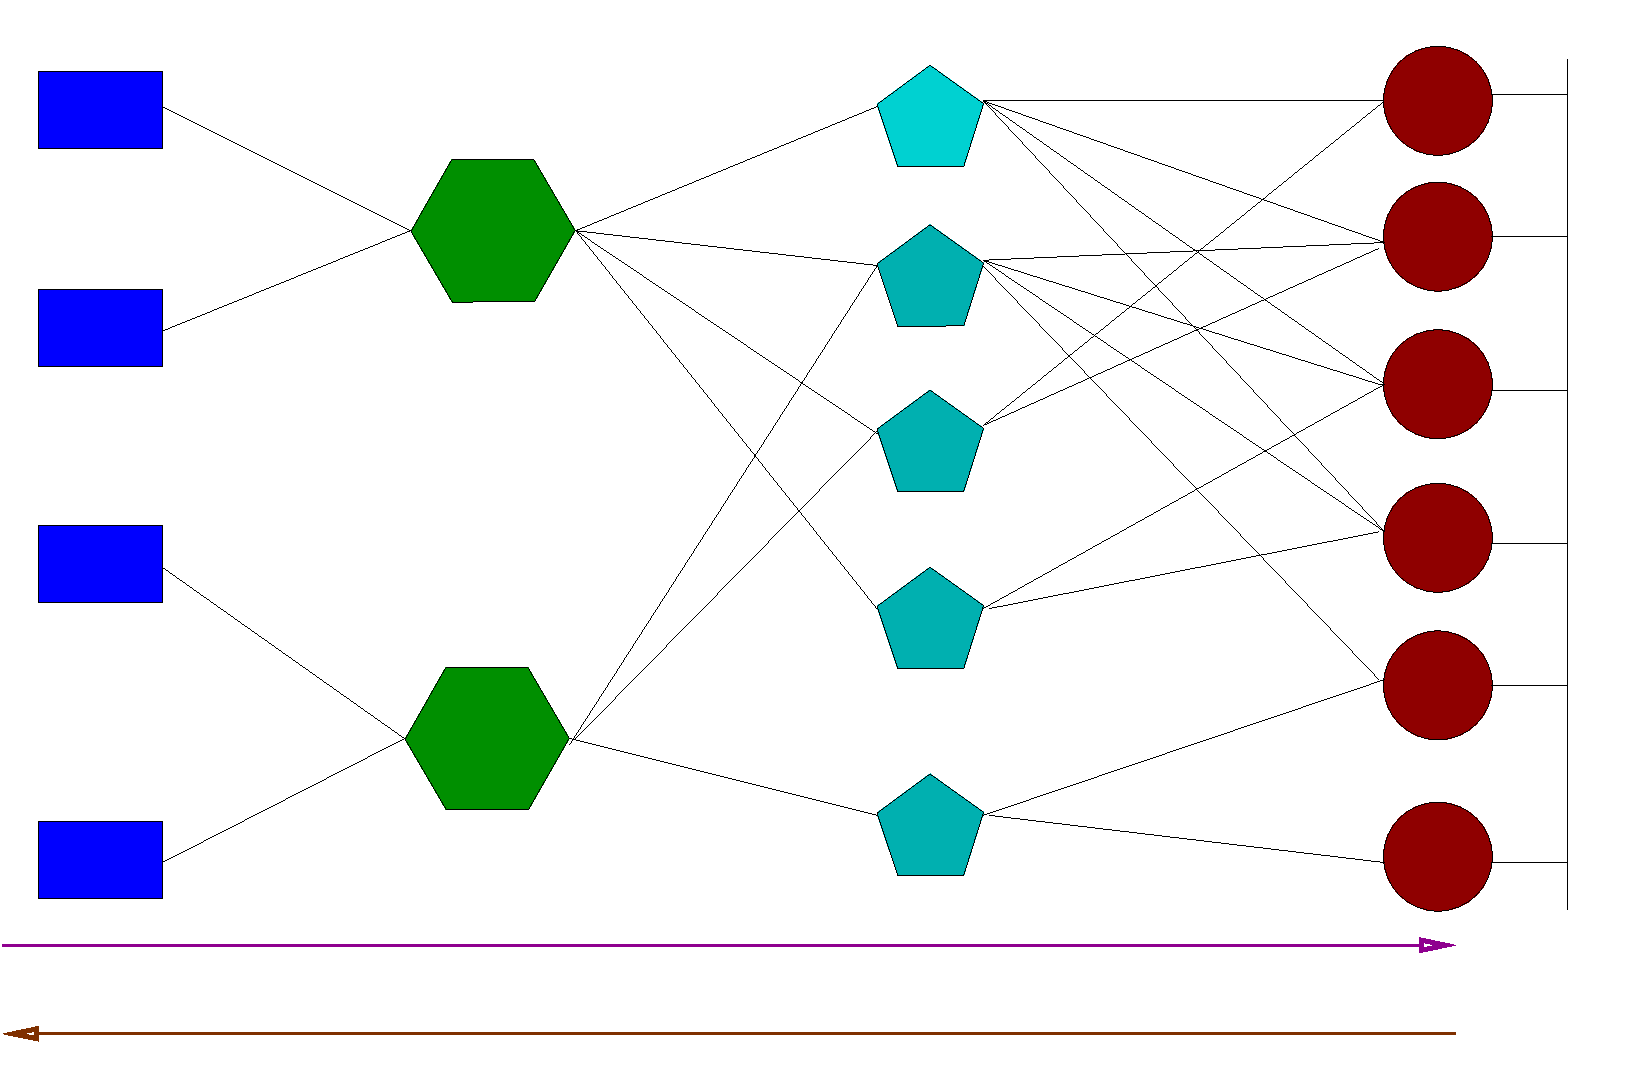
\includegraphics{sc/nodes1_color}%
\end{picture}%
\setlength{\unitlength}{4144sp}%
%
\begingroup\makeatletter\ifx\SetFigFont\undefined%
\gdef\SetFigFont#1#2#3#4#5{%
  \reset@font\fontsize{#1}{#2pt}%
  \fontfamily{#3}\fontseries{#4}\fontshape{#5}%
  \selectfont}%
\fi\endgroup%
\begin{picture}(12502,8244)(744,-8131)
\put(13231,-2626){\rotatebox{90.0}{\makebox(0,0)[rb]{\smash{{\SetFigFont{14}{16.8}{\rmdefault}{\mddefault}{\updefault}{\color[rgb]{0,0,0}CUSTOMERS}%
}}}}}
\put(9091,-7351){\makebox(0,0)[lb]{\smash{{\SetFigFont{17}{20.4}{\familydefault}{\mddefault}{\updefault}{\color[rgb]{.56,0,.56}Product Flow}%
}}}}
\put(946,-106){\makebox(0,0)[lb]{\smash{{\SetFigFont{17}{20.4}{\familydefault}{\mddefault}{\updefault}{\color[rgb]{0,0,1}Suppliers}%
}}}}
\put(7156,-106){\makebox(0,0)[lb]{\smash{{\SetFigFont{17}{20.4}{\familydefault}{\mddefault}{\updefault}{\color[rgb]{0,.69,.69}Distibution}%
}}}}
\put(7381,-331){\makebox(0,0)[lb]{\smash{{\SetFigFont{17}{20.4}{\familydefault}{\mddefault}{\updefault}{\color[rgb]{0,.69,.69}Centers}%
}}}}
\put(3826,-151){\makebox(0,0)[lb]{\smash{{\SetFigFont{17}{20.4}{\familydefault}{\mddefault}{\updefault}{\color[rgb]{0,.56,0}Production }%
}}}}
\put(4051,-511){\makebox(0,0)[lb]{\smash{{\SetFigFont{17}{20.4}{\familydefault}{\mddefault}{\updefault}{\color[rgb]{0,.56,0}Facility}%
}}}}
\put(11161,-106){\makebox(0,0)[lb]{\smash{{\SetFigFont{17}{20.4}{\familydefault}{\mddefault}{\updefault}{\color[rgb]{.56,0,0}Retailers}%
}}}}
\put(1396,-8116){\makebox(0,0)[lb]{\smash{{\SetFigFont{17}{20.4}{\familydefault}{\mddefault}{\updefault}{\color[rgb]{.5,.17,0}Information Flow}%
}}}}
\end{picture}%
}}
\caption{Supply chain as nodes and arcs.}
 \label{fig:sc:Nodes_and_Arcs}
\end{figure}

From a classical chemical engineering perspective, each node can be
modeled as two tanks, the inventory tank and the backorder tank. 
 The flows out of the inventory tank are the shipments
to the downstream nodes and the shipments from the upstream nodes make
up the flow into the inventory tank. The flows out of the backorder
tank are the shipments to the downstream nodes, which 
alternatively can be viewed as the orders that have been met; the
flows into the backorder tank are the orders arriving at the
node. For nodes that handle multiple products, we have as many
inventory and backorder tanks as the number of product handled by
the node.  Figure
\ref{fig:sc:nodemodel} depicts the `tanks' model of a node in the supply
chain handling a single product.
 \begin{figure}[h]
\centering
{\resizebox{0.75\textwidth}{!}{\begin{picture}(0,0)%
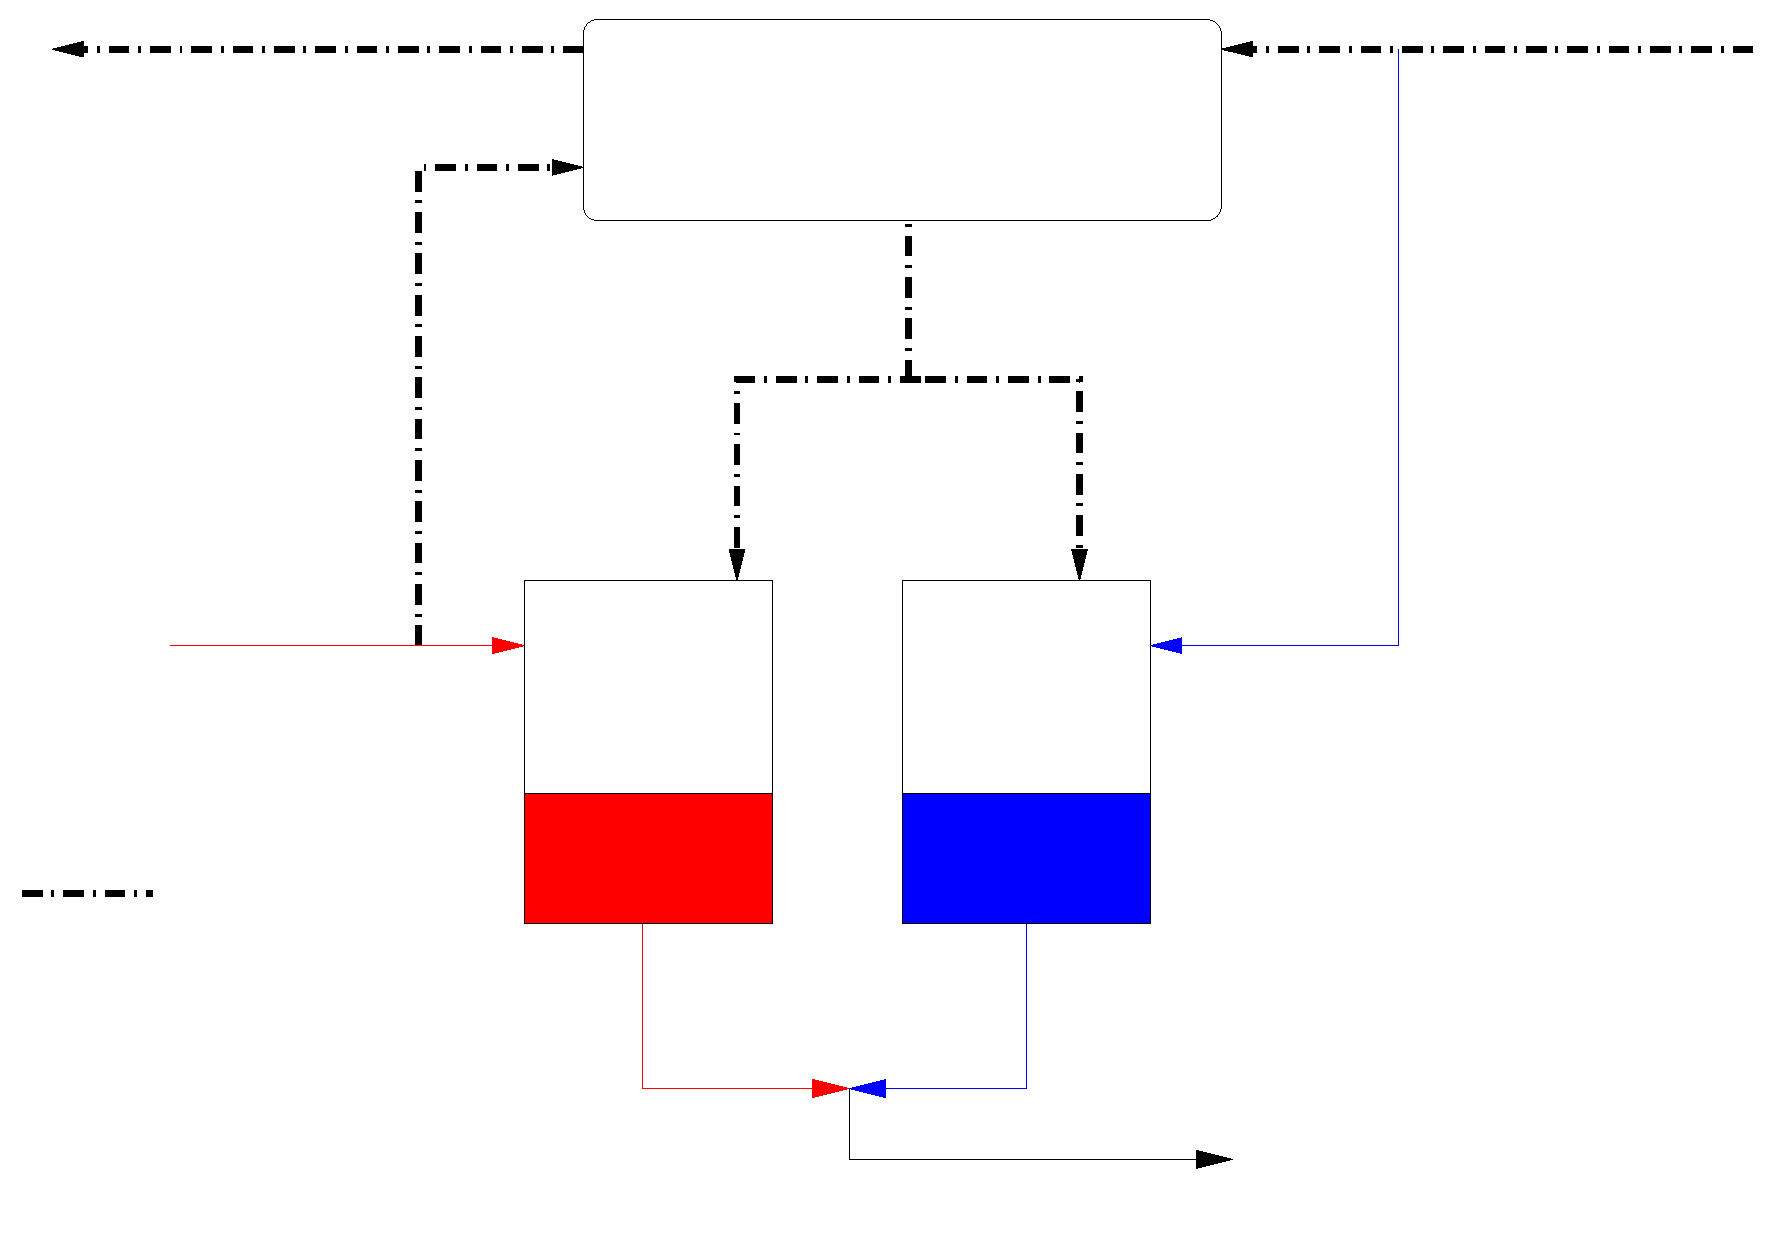
\includegraphics{model}%
\end{picture}%
\setlength{\unitlength}{4144sp}%
%
\begingroup\makeatletter\ifx\SetFigFont\undefined%
\gdef\SetFigFont#1#2#3#4#5{%
  \reset@font\fontsize{#1}{#2pt}%
  \fontfamily{#3}\fontseries{#4}\fontshape{#5}%
  \selectfont}%
\fi\endgroup%
\begin{picture}(13539,9207)(407,-8671)
\put(6841,-646){\makebox(0,0)[b]{\smash{{\SetFigFont{20}{24.0}{\rmdefault}{\mddefault}{\updefault}{\color[rgb]{0,0,0}(policy implementer/optimizer)}%
}}}}
\put(10486,-5191){\makebox(0,0)[lb]{\smash{{\SetFigFont{20}{24.0}{\rmdefault}{\mddefault}{\updefault}{\color[rgb]{0,0,0}Information sharing}%
}}}}
\put(4321,-4876){\makebox(0,0)[lb]{\smash{{\SetFigFont{20}{24.0}{\rmdefault}{\mddefault}{\updefault}{\color[rgb]{0,0,0}Inventory}%
}}}}
\put(7471,-5011){\makebox(0,0)[lb]{\smash{{\SetFigFont{20}{24.0}{\rmdefault}{\mddefault}{\updefault}{\color[rgb]{0,0,0}Orders}%
}}}}
\put(7471,-4696){\makebox(0,0)[lb]{\smash{{\SetFigFont{20}{24.0}{\rmdefault}{\mddefault}{\updefault}{\color[rgb]{0,0,0}Back-}%
}}}}
\put(721,-61){\makebox(0,0)[lb]{\smash{{\SetFigFont{20}{24.0}{\rmdefault}{\mddefault}{\updefault}{\color[rgb]{0,0,0}Orders}%
}}}}
\put(721,-361){\makebox(0,0)[lb]{\smash{{\SetFigFont{20}{24.0}{\rmdefault}{\mddefault}{\updefault}{\color[rgb]{0,0,0}(placed to }%
}}}}
\put(721,-661){\makebox(0,0)[lb]{\smash{{\SetFigFont{20}{24.0}{\rmdefault}{\mddefault}{\updefault}{\color[rgb]{0,0,0}upstream nodes)}%
}}}}
\put(11116,-61){\makebox(0,0)[lb]{\smash{{\SetFigFont{20}{24.0}{\rmdefault}{\mddefault}{\updefault}{\color[rgb]{0,0,0}Orders}%
}}}}
\put(11116,-376){\makebox(0,0)[lb]{\smash{{\SetFigFont{20}{24.0}{\rmdefault}{\mddefault}{\updefault}{\color[rgb]{0,0,0}(placed by}%
}}}}
\put(11116,-646){\makebox(0,0)[lb]{\smash{{\SetFigFont{20}{24.0}{\rmdefault}{\mddefault}{\updefault}{\color[rgb]{0,0,0}downstream nodes)}%
}}}}
\put(9676,-8566){\makebox(0,0)[lb]{\smash{{\SetFigFont{20}{24.0}{\rmdefault}{\mddefault}{\updefault}{\color[rgb]{0,0,0}(Demands satisfied)}%
}}}}
\put(9631,-8206){\makebox(0,0)[lb]{\smash{{\SetFigFont{20}{24.0}{\rmdefault}{\mddefault}{\updefault}{\color[rgb]{0,0,0}(to downstream nodes)}%
}}}}
\put(9631,-7846){\makebox(0,0)[lb]{\smash{{\SetFigFont{20}{24.0}{\rmdefault}{\mddefault}{\updefault}{\color[rgb]{0,0,0}Shipments }%
}}}}
\put(676,-4651){\makebox(0,0)[lb]{\smash{{\SetFigFont{20}{24.0}{\rmdefault}{\mddefault}{\updefault}{\color[rgb]{0,0,0}Shipments}%
}}}}
\put(676,-4951){\makebox(0,0)[lb]{\smash{{\SetFigFont{20}{24.0}{\rmdefault}{\mddefault}{\updefault}{\color[rgb]{0,0,0}(from upstream nodes)}%
}}}}
\put(6841,-196){\makebox(0,0)[b]{\smash{{\SetFigFont{20}{24.0}{\rmdefault}{\mddefault}{\updefault}{\color[rgb]{0,0,0}Decision Maker}%
}}}}
\end{picture}%
}}
\caption{Tank analogy for modeling a node.}
\label{fig:sc:nodemodel}
\end{figure}

The states in each node $i$ are:  the inventory in the node,
$\Inv_{pi} \forall p \in \mathcal{P}(i)$, and the backorders in the
node, $\BO_{pii'} \forall p \in \mathcal{P}(i), \forall i' \in \DN(i,p)$; two inputs:
the shipments made to each downstream node $j \in \DN(i,p)$, $S_{pij}$, and
the orders placed to each upstream node $j \in \UP(i,p)$, $O_{pij}$. The
shipments coming from the upstream nodes $S_{pji}, j \in \UP(i,p)$ and
the orders arriving from the downstream nodes $O_{pji}, j \in \DN(i,p)$
are the disturbances arriving to the node. Denoting discrete sample time by
integer $k$, the dynamic equations for node $i$ can be written as
\begin{align}
\Inv_{pi}(k+1) &= \Inv_{pi}(k) + \sum_{j \in \UP(i,p)}S_{pji}(k-\tau_{pji})
-\sum_{j \in \DN(i,p)}S_{pij}(k), \qquad \forall p \in \mathcal{P}(i)  \label{eq:sc:inventorybalance} \\
\BO_{pij}(k+1) &= \BO_{pij}(k) + O_{pji}(k) -S_{pij}(k),\qquad \forall
p \in \mathcal{P}(i), \forall j \in \DN(i,p)
\label{eq:sc:backorderbalance}
\end{align}
in which $\tau_{pji}$ is the transportation delay. We assume that there
are no delays for order transfers between the nodes.
Denoting $x_i(k) = \begin{bmatrix}\Inv_{pi}(k), p \in \mathcal{P}(i)  & \BO_{pij}(k),
   p \in \mathcal{P}(i),  j \in \DN(i,p)\end{bmatrix}'$,
$u_i(k) = \begin{bmatrix}S_{pij}, p \in \mathcal{P}(i), j \in \DN(i,p)&
  O_{pij'}, p \in \mathcal{P}(i),j' \in \UP(i,p)\end{bmatrix}'$, and
by using the lifting technique described in Chapter \ref{chap:scheduling},
the previous dynamic equations for the nodes
can be written in the familiar state space form for MPC applications 
\begin{equation}
x_i(k+1) = A_{ii}x_i(k) + B_{ii}u_i(k)+ \sum_{l\in\I \atop l \neq i}B_{il}u_l
%\label{eq:nodeequation}
\end{equation}
The decision maker shown in Figure \ref{fig:sc:nodemodel} can take
several different forms:
\begin{itemize}
\item Each decision maker can implement a simple ordering policy that
  depends only on the incoming shipments and orders. Such an ordering
  policy could be a PI controller to control the inventory levels, or
  $(\sigma,\Sigma)$ policies that are obtained from stochastic inventory
  control optimization. Such decision makers are implementations of
  classical control theory approaches to supply chain control.

\item {\textbf{Noncooperative MPC:}} Each decision maker can implement
  an MPC controller to regulate 
  its local states by optimizing a local objective function (for
  example, the profit function for the node). The nodes 
  can share information regarding upstream shipments,
  downstream orders, etc. This form of control is termed
  noncooperative MPC. 

\item {\textbf{Cooperative MPC:}} Each decision maker can implement an
  MPC controller  that 
  considers the effect of the nodes' decision on the entire supply chain
(for example, each node optimizes the supply chain profit
function). The nodes  still share information.

\item {\textbf{Centralized MPC:}} We can replace all the decision
  makers at the nodes with a 
  single decision maker at the supply chain level. This single
  decision maker  makes  decisions for all the nodes.
\end{itemize}  

The overall supply chain dynamic model is the individual node dynamic
equations  collected for all nodes $i \in \I$. The
only required change in the node dynamic equation
is for the retailer  and the production facility nodes.
\subsection*{Retailer models}
 For the retailer nodes $i \in \mathcal{R}$, the dynamic
equations are  modified as, 
\begin{align}
\Inv_{pi}(k+1) &= \Inv_i(k) + \sum_{j \in
  \UP(i,p)}S_{pji}(k-\tau_{pji}) - S_{pic}(k), \qquad \forall p \in \mathcal{P}(i)\\
\BO_{pi}(k+1) &= \BO_{pi}(k) + \Dem_{pic}(k)- S_{pic}(k),\qquad \forall p \in \mathcal{P}(i
\end{align}
in which $S_{pic}$ is the shipment made by the retailer, and
$\Dem_{pic}$ is the customer orders (demands).  \textit{The only disturbances in
the overall supply chain model are the customer demands} $d
= \begin{bmatrix} \Dem_{pic} \end{bmatrix}', p \in \mathcal{P}(i), i \in \mathcal{R}$, which
drive all the flows (shipments and orders) in the supply chain. 

\subsection*{Production facility models}

The production facility needs to be modeled separately because
material conversion takes place in this node. %The production facility model
%is the link between the raw material procurement dynamics and the finished
%product disbursement dynamics.
 In multiple product supply chains, the same production
facility handles multiple products. Thus a model for the production
facility needs to incorporate a scheduling model to optimize the
sequence of production. In this chapter, we assume that the production
facilities belong to  the first echelon. We further assume an ideal
supplier of raw materials to the production facilities, implying that
we have infinite supply of raw materials without transportation
delay. 

\paragraph{Planning models}
In this chapter, we shall use an ``approximate production model'' to 
model the production facility. In the approximate production model, we replace 
the detailed scheduling model with convex constraints that represent
the feasible region of production. This idea is similar to the process
attainable region \citep{sung:maravelias:2007}-a convex region of production
quantities for which there exists some feasible schedule. The process
attainable region can be computed by using computational geometry tools
\citep{sung:maravelias:2007, maravelias:sung:2009,
  sung:maravelias:2009} or parametric programming tools
\citep{li:ierapetritou:2010}. 
Let $\mathcal{M}$ be the set of production facility nodes. Then, for each $i \in \mathcal{M}$, the modified
dynamic equations for the final products are
\begin{align*}
\Inv_{pi}(k+1) &= \Inv_{pi}(k)+ S_{pim}(k) -\sum_{j \in
  \DN(i,p)}S_{pij}(k), \qquad \forall p \in \mathcal{P}(i)\\
\BO_{pij}(k+1) &= \BO_{pij}(k) + O_{pji}(k) -S_{pij}(k),\qquad \forall
p \in \mathcal{P}(i), \forall j \in \DN(i,p)
f(S_{ipm}(k)) &\leq 0
\end{align*}
in which $S_{pim}$ are the manipulated inputs denoting production of
product $p$  during the period. 
Note that, for multiproduct production facilities, each of the inputs
$S_{pim}$ for products $p \in \mathcal{P}$ are coupled by the
convex production feasibility constraint. The set $\mathcal{L}$
represents the set of products. 
\begin{equation*}
f(S_{1im}(k),S_{2ip}(k),\ldots,S_{pim}(k),\ldots) \leq 0
\end{equation*}


\paragraph{Scheduling models}
The state task network (STN) approach
is probably the most popular method to model a production facility in
which multiple products are produced using shared resources
\citep{kondili:pantelides:sargent:1993,shah:pantelides:sargent:1993}.
As described in Chapter \ref{chap:scheduling}, in STN modeling, the
final products, intermediates and raw materials are 
states that are processed using tasks like reactions, separation,
etc. These tasks can be carried out in units capable of
handling multiple tasks. A detailed schedule is the sequence of
operation of the tasks in the units so that a production objective
can be met at minimal cost without violating the scheduling
constraints.

Detailed scheduling models are formulated as mixed integer linear
programs (MILPs) or mixed integer nonlinear programs (MINLPs). If we
chose to model the production facility using a detailed scheduling
model, then the resulting supply chain MPC problems become mixed
integer programs. Although, research progress
has been made in the theory of MIQP and hybrid MPC (see
\citep{bemporad:morari:1999}), in this chapter, we do not consider
detailed scheduling models in the formulation of the supply
chain model. An example using a detailed scheduling model is provided
in Section \ref{sec:esc:multi}.


 

\subsection{Summary}
%\label{subsec:salient}
In this section, we wish to bring to the readers' attention, three
salient features of the supply chain dynamic model presented in this
section.

%\begin{enumerate}
%\item \textbf{Uncontrollable local models.} 
\paragraph{Uncontrollable local models} Controllability implies that there
  exist inputs that can move the state of the system from any initial
  state to any final state in finite time. Examining
  \eqref{eq:sc:inventorybalance} and \eqref{eq:sc:backorderbalance} for the 
  inventory and backorder balance  for node $i$, we observe that
  while nodes $j \in \UP(i,p)$ respond to orders $O_{pij}$ placed by node
  $i$, node $i$ has no knowledge of the subsequent dynamics of its own
  orders. Therefore, we need to provide the node 
  some model of how its orders affect the later shipments coming into the
  node. To do so in a noncooperative or decentralized control
  arrangement, we track another state (or output) $\IP_{pi}$ termed the
  inventory position. The dependence of orders on incoming
  shipments is modeled through the function $g(\cdot)$.
\begin{equation*}
\IP_{pi}(k+1) = \IP_{pi}(k) + \sum_{j \in \UP(i,p)}g(O_{pij}(k-\tau_{pji}))
- \sum_{j \in \DN(i)}S_{pij}(k) \qquad \forall p \in \mathcal{P}(i) 
\end{equation*}
In the centralized control framework, the actual dynamics of the entire
  supply chain is available to the decision maker, and the
  relationship of the orders at node $i$ to its subsequent incoming shipments is
  captured by the upstream nodes backorder balance equations and the
  supply chain performance metric. From Section
  \ref{sec:mpc:distributed:coop}, we know that cooperative MPC
  algorithms has complete model knowledge. Therefore, uncontrollable
  local models is not an issue when implementing cooperative MPC for
  supply chains.
\paragraph{Unstable models} The supply chain is
  modeled as a system of integrators whose
  response to an input step change is a ramp. Such systems
  need to be stabilized in the closed loop, otherwise the states can
  keep growing (think of it as backorders keep rising as time
  increases). Therefore, we emphasize establishing closed-loop
  properties 
  of the algorithms that we propose for supply chain optimization.
\paragraph{Stabilizable centralized model} We notice that all the
  nodes belonging to the manufacturing facilities are controllable
  because we manipulate the production rates. Therefore,  the
  manufacturing nodes do not require an inventory position
  model. Since the manufacturing 
  facility model has this property, the overall supply chain model is
  also controllable. The controllability of the centralized model is an
  important feature that we use to design closed-loop stable
  centralized and cooperative MPC frameworks for supply chain
  optimization.

\section{Example\footnote{The results this section, with the exception of
Sections \ref{sec:sc:supplycahin_example:robust},
\ref{sec:sc:supplychain_example:lssc} and the discussion on steady states, are slightly modified from Section 6 of
\citet{subramanian:rawlings:maravelias:2012} to reflect a coding error
that was corrected. }}
\label{sec:sc:supplychain_example}
We simulate the supply chain shown in Figure \ref{fig:sc:2stage} in this
section. The plant  has production delay of 2 time units and a
transportation delay of 2 time units and a single product. For
simplicity, we drop the index on product in this section. 

\paragraph{Production model}
As mentioned earlier, the production delay is 2 time units. However,
we assume that the manufacturer can start a batch of the product at
every sampling time. This assumption means that the manufacturer has
two units that can execute the task of producing the final product. 

\begin{figure}
\centering
\resizebox{0.75\textwidth}{!}{\begin{picture}(0,0)%
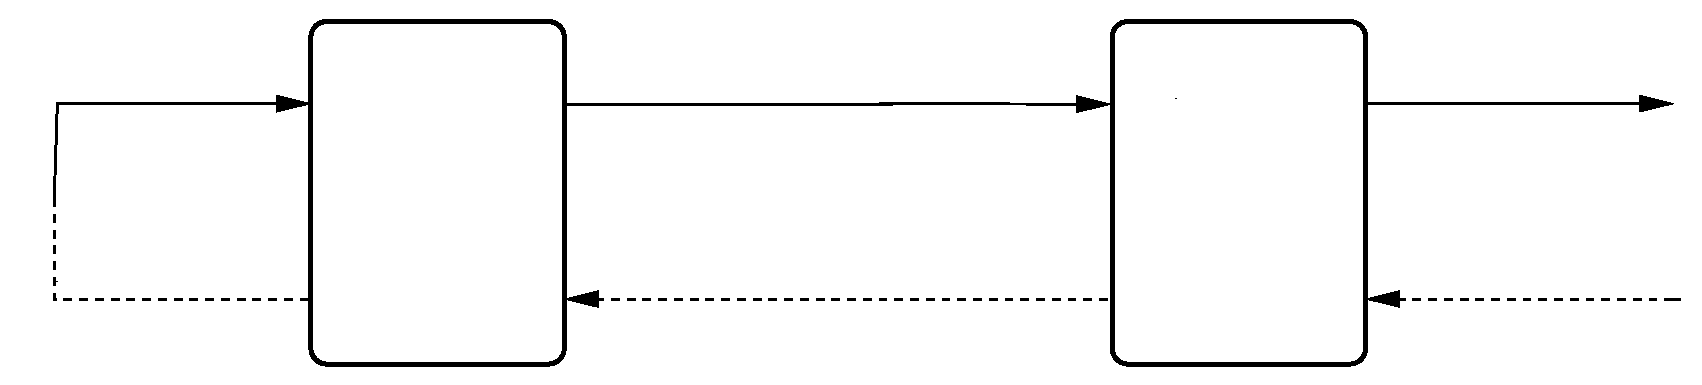
\includegraphics{sc/2node}%
\end{picture}%
\setlength{\unitlength}{4144sp}%
%
\begingroup\makeatletter\ifx\SetFigFont\undefined%
\gdef\SetFigFont#1#2#3#4#5{%
  \reset@font\fontsize{#1}{#2pt}%
  \fontfamily{#3}\fontseries{#4}\fontshape{#5}%
  \selectfont}%
\fi\endgroup%
\begin{picture}(10914,2274)(1114,-4123)
\put(1936,-3796){\makebox(0,0)[lb]{\smash{{\SetFigFont{12}{14.4}{\familydefault}{\mddefault}{\updefault}{\color[rgb]{0,0,0}$S_{2p}(k)$}%
}}}}
\put(11116,-3841){\makebox(0,0)[lb]{\smash{{\SetFigFont{12}{14.4}{\familydefault}{\mddefault}{\updefault}{\color[rgb]{0,0,0}$dem_{1c}(k)$}%
}}}}
\put(1576,-2266){\makebox(0,0)[lb]{\smash{{\SetFigFont{12}{14.4}{\familydefault}{\mddefault}{\updefault}{\color[rgb]{0,0,0}$S_{2p}(k-\tau_M)$}%
}}}}
\put(3106,-2986){\makebox(0,0)[lb]{\smash{{\SetFigFont{14}{16.8}{\familydefault}{\mddefault}{\updefault}{\color[rgb]{0,0,0}Manufacturer}%
}}}}
\put(8641,-2986){\makebox(0,0)[lb]{\smash{{\SetFigFont{14}{16.8}{\familydefault}{\mddefault}{\updefault}{\color[rgb]{0,0,0}Retailer}%
}}}}
\put(6166,-2491){\makebox(0,0)[lb]{\smash{{\SetFigFont{10}{12.0}{\familydefault}{\mddefault}{\updefault}{\color[rgb]{0,0,0}$\tau_T=2$}%
}}}}
\put(1171,-3031){\makebox(0,0)[lb]{\smash{{\SetFigFont{10}{12.0}{\familydefault}{\mddefault}{\updefault}{\color[rgb]{0,0,0}$\tau_M = 2$}%
}}}}
\put(8686,-3301){\makebox(0,0)[lb]{\smash{{\SetFigFont{12}{14.4}{\familydefault}{\mddefault}{\updefault}{\color[rgb]{0,0,0}Node $1$}%
}}}}
\put(9991,-2311){\makebox(0,0)[lb]{\smash{{\SetFigFont{12}{14.4}{\familydefault}{\mddefault}{\updefault}{\color[rgb]{0,0,0}$S_{1c}(k)$}%
}}}}
\put(7201,-3886){\makebox(0,0)[lb]{\smash{{\SetFigFont{12}{14.4}{\familydefault}{\mddefault}{\updefault}{\color[rgb]{0,0,0}$O_{12}(k)$}%
}}}}
\put(4816,-2716){\makebox(0,0)[lb]{\smash{{\SetFigFont{12}{14.4}{\familydefault}{\mddefault}{\updefault}{\color[rgb]{0,0,0}$S_{21}(k)$}%
}}}}
\put(3421,-3301){\makebox(0,0)[lb]{\smash{{\SetFigFont{12}{14.4}{\familydefault}{\mddefault}{\updefault}{\color[rgb]{0,0,0}Node $2$}%
}}}}
\end{picture}%
}
\caption{Two-stage supply chain.}
\label{fig:sc:2stage}
\end{figure}
We label the retailer node $1$, with the states $\Inv_1$ and
$\BO_1$, the inventory and backorder at the retailer. The retailer
inputs $u_1$ consist of orders placed  and the shipments made by the retailer, $S_{1c}$ and
$O_{12}$.
We label the manufacturer  node $2$, with states $x_2$ consisting of
inventory $\Inv_2$ and backorder $\BO_2$. The manufacturer inputs
are the shipments made to the retailer $S_{21}$ and the production
e$S_{2m}$.  The demand $d(k) = \Dem_{1c}$. 

\paragraph{Models}
We write a  time invariant model  for the supply chain that is also the
 process model (because we assume that a batch may start at every
 time) by writing the inventory and backorder balance equation. These
 model for the retailer is:
\begin{equation}
\label{eq:sc:scheduling_example:R}
\underbrace{\begin{bmatrix}\Inv_1\\\BO_1\end{bmatrix}_{k+1}}_{x_1(k+1)} =
\underbrace{\begin{bmatrix}1&\\ &
    1\end{bmatrix}}_{A_1}\underbrace{\begin{bmatrix}\Inv_1\\\BO_1\end{bmatrix}_k}_{x_1(k)}
+\underbrace{\begin{bmatrix}-1 & 0 \\-1&
    0 \end{bmatrix}}_{B_{11}}\underbrace{\begin{bmatrix}S_{1c}\\O_{12}\end{bmatrix}_k}_{u_1(k)}
+\underbrace{\begin{bmatrix}-1 & 0 \\0&
    0 \end{bmatrix}}_{B_{22}^{(2)}}\underbrace{\begin{bmatrix}S_{21}\\S_{2m}\end{bmatrix}_{k-2}}_{u_2(k-2)}
+\underbrace{\begin{bmatrix} 0\\1\end{bmatrix}}_{B_d}\underbrace{\begin{bmatrix}\Dem_{1c}\end{bmatrix}_{k}}_{d(k)}
\end{equation}

The manufacturer state space is given by:
\begin{equation}
\label{eq:sc:scheduling_example:M}
\underbrace{\begin{bmatrix}\Inv_2\\\BO_2\end{bmatrix}_{k+1}}_{x_2(k+1)} =
\underbrace{\begin{bmatrix}1&\\ &
    1\end{bmatrix}}_{A_2}\underbrace{\begin{bmatrix}\Inv_2\\\BO_2\end{bmatrix}_k}_{x_2(k)}
+\underbrace{\begin{bmatrix}-1 & 0 \\-1&
    0 \end{bmatrix}}_{B_{22}}\underbrace{\begin{bmatrix}S_{21}\\S_{2m}\end{bmatrix}_k}_{u_2(k)}
+\underbrace{\begin{bmatrix}0 & 1 \\0&
    0 \end{bmatrix}}_{B_{22}^{(2)}}\underbrace{\begin{bmatrix}S_{21}\\S_{2m}\end{bmatrix}_{k-2}}_{u_2(k-2)}
+\underbrace{\begin{bmatrix} 0 & 0 \\0 &1\end{bmatrix}}_{B_{12}}\underbrace{\begin{bmatrix}S_{1c}\\O_{12}\end{bmatrix}_{k}}_{u_1(k)}
\end{equation}

Notice that the retailer, by just using $u_1$ cannot move the states
from any initial condition to any final condition. We can easily
verify this using the Hautus lemma. This matrix $\begin{bmatrix} I-A_1 & B_{11} \end{bmatrix}$ is
rank-deficient. 

\paragraph{Steady state} From equations
\eqref{eq:sc:scheduling_example:R} and
\eqref{eq:sc:scheduling_example:M}, we notice that if $B_{11}u_1(k) + B_{21}^{(2)}u_2(k-2)+B_dd(k) = 0$ and
$B_{22}u_2(k)+B_{22}^{(2)}u_2(k-2)+B_{12}u_1(k) = 0$, then any
inventory and backorder level can be a steady-state. From the tanks
analogy, as long as all the flows in and out of the tank are equal,
any level inside the tank is steady. Hence, we have a degree of
freedom in choosing the steady state for the inventories and backorders. The steady states
for the inputs is determined by the nominal (steady state) demand. Since, we wish to
meet all demands, the steady state for backorders is zero. On the
other hand, we wish to maintain a safety stock, and so we
choose inventory targets to regulate around. In the discussion that follows, we use
$x$ to denote deviation from the steady state, i.e., we redefine $x
\leftarrow x-x_s$ in which $x_s =
(\Inv_{1,t},0,\Inv_{2,t},0)$, with $\Inv_t$ referring
to the inventory target.


\paragraph{Stage cost}
Each node (subsystem) has a local stage cost, given by
\begin{equation*}
\ell_1(x_1,u_1)  = \norm{x_1}^2_{Q_1} + \norm{u_1}^2_{R_1},\quad
\ell_2(x_2,u_2) = \norm{x_2}^2_{Q_2} + \norm{u_2}^2_{R_2}
\end{equation*}
The overall stage cost is $\ell(x,u) =
\ell_1(x_1,u_1)+\ell_2(x_2,u_2)$. The costs used are $Q_1=Q_2=
\diag(1,10)$ and $R_1=R_2 = diag(1,1)$.

\paragraph{Terminal cost}
For centralized and cooperative MPC, following the theory outlined in
Section \ref{sec:mpc:distributed:relaxation}, we chose the $P>0,a>0$ such that there exists a
stabilizing control law $\kappa_f(x)$ in the terminal region given by:
\begin{equation*}
\mathbb{X}_f = \lbrace x \mid x'Px \leq a \rbrace
\end{equation*}
We also choose a $\bar{V}>0$ and fix $\beta = \max{(1,\bar{V}/a)}$. The
positive definite matrix $P$ is of the form $\left[ \begin{smallmatrix}P_{11}&
  P_{12} \\ P_{12}' & P_{22}\end{smallmatrix} \right]$. We choose the local
terminal cost functions and the centralized terminal cost function as 
\begin{equation*}
V_f^{1}(x_1) = \norm{x_1}_{P_{11}}^2 \qquad 
%\label{eq:terminal_R}
%\end{equation*}
%\begin{equation*}
V_f^{2}(x_2) = \norm{x_2}_{P_{22}}^2 \qquad
%\label{eq:terminal_M}
%\end{equation*}
%and the centralized cost function
%\begin{equation*}
V_f(x) = \norm{x}_P^2
%\label{eq:terminal_C}
\end{equation*}

We now define the MPC cost functions. The subsystem cost functions
are for $i \in \lbrace 1,2 \rbrace$
\begin{equation*}
V_N^{i,\beta}(x_i(0),\bu_i) =
\sum_{j=0}^{N-1}\ell_i(x_i(j),u_i(j)) \\ 
+ \beta V_f^{i}(x_i(N))
\end{equation*}
while the overall cost function is:
\begin{equation*}
V_N^\beta(x,\bu) = \sum_{j=0}^{N-1}\ell(x(j),u(j)) + \beta V_f(x(N))
\end{equation*}
Note that since we defined the terminal costs differently for the
subsystems, the overall cost function 
is not the sum of the subsystem cost functions. 
Associated with each input, we also have the input constraint set
$\mathbb{U}_1$ and $\mathbb{U}_2$, which contain the minimum and maximum
shipments and orders that can flow through the supply chain. The
maximum shipment allowed was capped at $40$ units, while any positive
order could be placed (arbitrarily large constraint).

\subsection*{MPC implementation}
\paragraph{Ordering policies}
As mentioned in Section \ref{sec:sc:modeling}, the local retailer model
does not have knowledge of how the orders placed by the retailer
affects the supply chain. Therefore, in the implementation of
noncooperative and decentralized MPC, we need to incorporate an
ordering policy for the retailer. Since the manufacturer reacts to the
orders placed by the retailer, the closed-loop performance of the
supply chain is intimately connected to the ordering policy.
We study two ordering policies in this example:
\begin{enumerate}
\item Order-up-to policy: The order-up-to  policy can be viewed as a
  saturated proportional  controller.
\begin{equation}
    O_{12}(k) = \begin{cases} \Inv_t-\Inv_1(k) & \text{if $\Inv_1 \leq \Inv_t$} \\
            0 & \text{otherwise}  \end{cases}
\end{equation}
in which $\Inv_t$ is the inventory target.
 
\item Inventory position control: In inventory position control, the
  retailer, instead of controlling the inventory, controls the
  inventory position, which is a controlled output defined as:
 \begin{equation}
   \IP(k) = \Inv_1(k)-S_{1c}(k) + O_{12}(k)
  \end{equation}
  Inventory position control introduces a new
  controlled output that is a function of the state and input. We
  penalize the deviations of $\IP$ from the inventory target
  $\Inv_t$ in the optimizations.
\end{enumerate}

\paragraph{Distributed MPC}
In decentralized and noncooperative MPC with order-up-to policy, we
modify the retailer subproblem, subsystem-1  in \eqref{eq:mpc:distributed:ncoop:PNi},
by adding a constraint that enforces the order-up-to
policy. Similarly, for decentralized and noncooperative MPC with
inventory position control, we modify the retailer objective function
in the  subsystem-1 problem in \eqref{eq:mpc:distributed:ncoop:PNi} by
modifying the stage cost to penalize inventory position $\IP$. We
present the optimization problem  \eqref{eq:mpc:distributed:ncoop:PNi}
again here for convenience (Note that (i) We do not have state constraints
in this example following Assumption \ref{ass:mpc:noX}, (ii) the
terminal penalty is magnified using the parameter $\beta$.)
\begin{xalignat*}{2}
\mathbb{P}_{N,nc}^i(x_i;\mathbf{v}_{-i}):& \min_{\bu_i}{\sum_{j=0}^{N-1}
\ell_i(x_i(j),u_i(j)) +\beta V_{f,i}(x_i(N))}& \nonumber\\
&\text{s.t.~} x_i(j+1) = Ax_i(j) + Bu_i(j) +  \sum_{l \in \set{1,2,\ldots,M} \atop l \neq i}
B_{li} v_l(j) & j = \set{0,1,\ldots,N-1} \nonumber\\
& u_i(j) \in \mathbb{U}_i & j = \set{0,1,\ldots,N-1} \nonumber \\
&x_i(0) = x_i \nonumber
\end{xalignat*}


Decentralized and noncooperative MPC are implemented using Algorithm
\ref{alg:mpc:distributed:ncoop}. In decentralized MPC, the subsystems do not share
information. That is $\mathbf{\nu}_{-i}$ is assumed by each subsystem
to makes its local predictions. Therefore, in the supply chain
context, we add another source of inaccuracy with decentralized
control (to add to using ordering policies).


The subproblems for cooperative MPC are obtained by fixing the other
subsystem inputs in the centralized optimization
problem \label{eq:mpc:distributed:relaxation:PNx} (reproduced here for convenience). Cooperative MPC
is implemented using Algorithm \ref{alg:mpc:distributed:coop}. In centralized MPC, we
solve the overall problem $\mathbb{P}^\beta_N(x)$ given in
\eqref{eq:mpc:distributed:relaxation:PNx}. The parameter $\beta$ was
chosen as $1000$. 

\begin{xalignat*}{2}
\mathbb{P}_N(x):& \min_{\bu}V^\beta_N(x,\bu) & \nonumber \\
&\text{s.t.~} x(j+1) = Ax(j) + Bu(j), &  j =
\set{1,2,\ldots,N-1} \nonumber \\
&u(j) \in \mathbb{U} &  j =
\set{0,1,2,\ldots,N-1} \nonumber \\
&x(0) = x & \nonumber\\
\end{xalignat*}

\subsection{Nominal demands}
\label{sec:sc:supplychain_example:nominal}
We present the results of the different MPC
implementations for a nominal demand of $d = 8$. In each of the
simulations, the retailer starts with inventory $\Inv_1 = 47$ and the
manufacturer starts with inventory $\Inv_2 = 32$. The control objective
is to keep the inventories in the nodes as close to the target
inventory ($\Inv_1 = 45$ and $\Inv_2 = 30$)as possible while maintaining minimum backorder. 

Figure \ref{fig:sc:orderupto} compares the results of centralized,
cooperative, noncooperative and decentralized MPC in which we used the
order-up-to ordering policy.  Figure \ref{fig:sc:IP_x} compares the
results of same controllers, but using the inventory control policy.
\begin{figure}
\centering
\scriptsize
\resizebox{\textwidth}{!}{\input{sc/sS_demand}}
\resizebox{\textwidth}{!}{\input{sc/sS_demand_input}}
\caption{Inventories and orders placed in the supply chain: Order-up-to policy (dec:
  decentralized, ncoop: noncooperative, coop: cooperative, cent: centralized).}
\label{fig:sc:orderupto}
\end{figure}

\begin{figure}
\centering
\scriptsize
\resizebox{\textwidth}{!}{% GNUPLOT: LaTeX picture with Postscript
\begingroup
  \makeatletter
  \providecommand\color[2][]{%
    \GenericError{(gnuplot) \space\space\space\@spaces}{%
      Package color not loaded in conjunction with
      terminal option `colourtext'%
    }{See the gnuplot documentation for explanation.%
    }{Either use 'blacktext' in gnuplot or load the package
      color.sty in LaTeX.}%
    \renewcommand\color[2][]{}%
  }%
  \providecommand\includegraphics[2][]{%
    \GenericError{(gnuplot) \space\space\space\@spaces}{%
      Package graphicx or graphics not loaded%
    }{See the gnuplot documentation for explanation.%
    }{The gnuplot epslatex terminal needs graphicx.sty or graphics.sty.}%
    \renewcommand\includegraphics[2][]{}%
  }%
  \providecommand\rotatebox[2]{#2}%
  \@ifundefined{ifGPcolor}{%
    \newif\ifGPcolor
    \GPcolortrue
  }{}%
  \@ifundefined{ifGPblacktext}{%
    \newif\ifGPblacktext
    \GPblacktexttrue
  }{}%
  % define a \g@addto@macro without @ in the name:
  \let\gplgaddtomacro\g@addto@macro
  % define empty templates for all commands taking text:
  \gdef\gplbacktext{}%
  \gdef\gplfronttext{}%
  \makeatother
  \ifGPblacktext
    % no textcolor at all
    \def\colorrgb#1{}%
    \def\colorgray#1{}%
  \else
    % gray or color?
    \ifGPcolor
      \def\colorrgb#1{\color[rgb]{#1}}%
      \def\colorgray#1{\color[gray]{#1}}%
      \expandafter\def\csname LTw\endcsname{\color{white}}%
      \expandafter\def\csname LTb\endcsname{\color{black}}%
      \expandafter\def\csname LTa\endcsname{\color{black}}%
      \expandafter\def\csname LT0\endcsname{\color[rgb]{1,0,0}}%
      \expandafter\def\csname LT1\endcsname{\color[rgb]{0,1,0}}%
      \expandafter\def\csname LT2\endcsname{\color[rgb]{0,0,1}}%
      \expandafter\def\csname LT3\endcsname{\color[rgb]{1,0,1}}%
      \expandafter\def\csname LT4\endcsname{\color[rgb]{0,1,1}}%
      \expandafter\def\csname LT5\endcsname{\color[rgb]{1,1,0}}%
      \expandafter\def\csname LT6\endcsname{\color[rgb]{0,0,0}}%
      \expandafter\def\csname LT7\endcsname{\color[rgb]{1,0.3,0}}%
      \expandafter\def\csname LT8\endcsname{\color[rgb]{0.5,0.5,0.5}}%
    \else
      % gray
      \def\colorrgb#1{\color{black}}%
      \def\colorgray#1{\color[gray]{#1}}%
      \expandafter\def\csname LTw\endcsname{\color{white}}%
      \expandafter\def\csname LTb\endcsname{\color{black}}%
      \expandafter\def\csname LTa\endcsname{\color{black}}%
      \expandafter\def\csname LT0\endcsname{\color{black}}%
      \expandafter\def\csname LT1\endcsname{\color{black}}%
      \expandafter\def\csname LT2\endcsname{\color{black}}%
      \expandafter\def\csname LT3\endcsname{\color{black}}%
      \expandafter\def\csname LT4\endcsname{\color{black}}%
      \expandafter\def\csname LT5\endcsname{\color{black}}%
      \expandafter\def\csname LT6\endcsname{\color{black}}%
      \expandafter\def\csname LT7\endcsname{\color{black}}%
      \expandafter\def\csname LT8\endcsname{\color{black}}%
    \fi
  \fi
  \setlength{\unitlength}{0.0500bp}%
  \begin{picture}(7200.00,3024.00)%
    \gplgaddtomacro\gplbacktext{%
      \csname LTb\endcsname%
      \put(814,440){\makebox(0,0)[r]{\strut{}-20}}%
      \put(814,1020){\makebox(0,0)[r]{\strut{} 0}}%
      \put(814,1600){\makebox(0,0)[r]{\strut{} 20}}%
      \put(814,2179){\makebox(0,0)[r]{\strut{} 40}}%
      \put(814,2759){\makebox(0,0)[r]{\strut{} 60}}%
      \put(946,220){\makebox(0,0){\strut{} 0}}%
      \put(1433,220){\makebox(0,0){\strut{} 10}}%
      \put(1921,220){\makebox(0,0){\strut{} 20}}%
      \put(2408,220){\makebox(0,0){\strut{} 30}}%
      \put(2896,220){\makebox(0,0){\strut{} 40}}%
      \put(3383,220){\makebox(0,0){\strut{} 50}}%
      \put(176,1599){\rotatebox{-270}{\makebox(0,0){\strut{}Inventory-Retailer}}}%
    }%
    \gplgaddtomacro\gplfronttext{%
      \csname LTb\endcsname%
      \put(2396,833){\makebox(0,0)[r]{\strut{}dec}}%
      \csname LTb\endcsname%
      \put(2396,613){\makebox(0,0)[r]{\strut{}ncoop}}%
    }%
    \gplgaddtomacro\gplbacktext{%
      \csname LTb\endcsname%
      \put(4109,220){\makebox(0,0){\strut{} 0}}%
      \put(4544,220){\makebox(0,0){\strut{} 10}}%
      \put(4978,220){\makebox(0,0){\strut{} 20}}%
      \put(5413,220){\makebox(0,0){\strut{} 30}}%
      \put(5847,220){\makebox(0,0){\strut{} 40}}%
      \put(6282,220){\makebox(0,0){\strut{} 50}}%
      \put(6414,440){\makebox(0,0)[l]{\strut{} 0}}%
      \put(6414,827){\makebox(0,0)[l]{\strut{} 10}}%
      \put(6414,1213){\makebox(0,0)[l]{\strut{} 20}}%
      \put(6414,1600){\makebox(0,0)[l]{\strut{} 30}}%
      \put(6414,1986){\makebox(0,0)[l]{\strut{} 40}}%
      \put(6414,2373){\makebox(0,0)[l]{\strut{} 50}}%
      \put(6414,2759){\makebox(0,0)[l]{\strut{} 60}}%
      \put(7051,1599){\rotatebox{-270}{\makebox(0,0){\strut{}Inventory-Manufacturer}}}%
    }%
    \gplgaddtomacro\gplfronttext{%
      \csname LTb\endcsname%
      \put(5295,833){\makebox(0,0)[r]{\strut{}coop}}%
      \csname LTb\endcsname%
      \put(5295,613){\makebox(0,0)[r]{\strut{}cent}}%
    }%
    \gplbacktext
    \put(0,0){\includegraphics{sc/IP_dem}}%
    \gplfronttext
  \end{picture}%
\endgroup
}
\resizebox{\textwidth}{!}{\input{sc/IP_dem_input}}
\caption{Inventories and orders placed in the supply chain: Inventory position control (dec:
  decentralized, ncoop: noncooperative, coop: cooperative, cent: centralized).}
\label{fig:sc:IP_x}
\end{figure}

We defer discussion about the results to Section \ref{sec:sc:discussion}

\subsection{Stochastic demands}
\label{sec:sc:supplycahin_example:robust}
In \ref{sec:sc:supplychain_example:nominal}, we showed the response
using a model predictive controller for a supply chain observing
nominal demands. In this section, we show the results of implementing
the robust MPC algorithm presented in Section \ref{sec:mpc:robust}. We
consider the two node supply chain shown in Figure
\ref{fig:sc:2stage}, but with a nominal demand of $10$ units per time
period. The demand is assumed to be stochastic between $5$ and $15$
units per time period. In this example, we choose the retailer target
inventory $\Inv_{1,t} = 35$. 

Following the procedure outlined in Section \ref{sec:mpc:robust}, we
(i) design a stable cooperative MPC for the nominal system using the
methods outlined in the previous section, but with the tightened input
constraint sets to account for stochastic demands, and (ii) use the terminal
controller $\kappa_f(x) = Kx$ to account for the stochasticity in
demand. We used the technique outlined in \citet{rao:rawlings:1999} to find
$\kappa_f(x) = Kx$, such that all outstanding orders (backlogged
demands) from the previous time (if any) are satisfied at the current
sampling time. We chose the gain $K$ such that
$(A+BK)e$ implied that error in the backorder state was zero. Recall
that $e(k) = x(k)-z(k)$; the deviation between the actual state and
the nominal state. Hence, there is a delay
of 1 sampling time before the system reacts to the stochastic
demands. 


In Figure \ref{fig:sc:supplychain_example:CL1}, we show the closed-loop response 
nominal closed-loop response of the  inventory at the retailer for
cooperative MPC responding to a stochastic demand signal.  We also show the cost-function $V^\beta_N(z,\tilde{\mathbf{v}})$ and
$V^\beta_N(x,\tilde{\mathbf{v}})$ to show that although the warm-start was
infeasible for the actual state, it was still feasible for the nominal
state and hence we could obtain the closed-loop guarantees for robust
cooperative MPC. We used $\bar{V} = 20000$. Hence, whenever the cost
function for the actual state was greater than $20000$, it meant that
the warm-start was infeasible. That is, the terminal state was not
inside the set $\mathbb{X}_f$. However, by design of cooperative
algorithm, the warm start always remains feasible for the nominal MPC
problem.

In Figure \ref{fig:sc:supplychain_example:CL2}, we show the closed-loop response using a
modified version of Algorithm \ref{alg:mpc:robust} discussed in Section \ref{sec:mpc:robust}.

\begin{figure}
\centering
\scriptsize
\resizebox{\textwidth}{!}{\input{sc/CL1}}
\caption{(Left) Closed-loop response (Right) Warm start rendered
  infeasible for actual state because of disturbance}
\label{fig:sc:supplychain_example:CL1}
\centering
\scriptsize
\resizebox{\textwidth}{!}{% GNUPLOT: LaTeX picture with Postscript
\begingroup
  \makeatletter
  \providecommand\color[2][]{%
    \GenericError{(gnuplot) \space\space\space\@spaces}{%
      Package color not loaded in conjunction with
      terminal option `colourtext'%
    }{See the gnuplot documentation for explanation.%
    }{Either use 'blacktext' in gnuplot or load the package
      color.sty in LaTeX.}%
    \renewcommand\color[2][]{}%
  }%
  \providecommand\includegraphics[2][]{%
    \GenericError{(gnuplot) \space\space\space\@spaces}{%
      Package graphicx or graphics not loaded%
    }{See the gnuplot documentation for explanation.%
    }{The gnuplot epslatex terminal needs graphicx.sty or graphics.sty.}%
    \renewcommand\includegraphics[2][]{}%
  }%
  \providecommand\rotatebox[2]{#2}%
  \@ifundefined{ifGPcolor}{%
    \newif\ifGPcolor
    \GPcolortrue
  }{}%
  \@ifundefined{ifGPblacktext}{%
    \newif\ifGPblacktext
    \GPblacktexttrue
  }{}%
  % define a \g@addto@macro without @ in the name:
  \let\gplgaddtomacro\g@addto@macro
  % define empty templates for all commands taking text:
  \gdef\gplbacktext{}%
  \gdef\gplfronttext{}%
  \makeatother
  \ifGPblacktext
    % no textcolor at all
    \def\colorrgb#1{}%
    \def\colorgray#1{}%
  \else
    % gray or color?
    \ifGPcolor
      \def\colorrgb#1{\color[rgb]{#1}}%
      \def\colorgray#1{\color[gray]{#1}}%
      \expandafter\def\csname LTw\endcsname{\color{white}}%
      \expandafter\def\csname LTb\endcsname{\color{black}}%
      \expandafter\def\csname LTa\endcsname{\color{black}}%
      \expandafter\def\csname LT0\endcsname{\color[rgb]{1,0,0}}%
      \expandafter\def\csname LT1\endcsname{\color[rgb]{0,1,0}}%
      \expandafter\def\csname LT2\endcsname{\color[rgb]{0,0,1}}%
      \expandafter\def\csname LT3\endcsname{\color[rgb]{1,0,1}}%
      \expandafter\def\csname LT4\endcsname{\color[rgb]{0,1,1}}%
      \expandafter\def\csname LT5\endcsname{\color[rgb]{1,1,0}}%
      \expandafter\def\csname LT6\endcsname{\color[rgb]{0,0,0}}%
      \expandafter\def\csname LT7\endcsname{\color[rgb]{1,0.3,0}}%
      \expandafter\def\csname LT8\endcsname{\color[rgb]{0.5,0.5,0.5}}%
    \else
      % gray
      \def\colorrgb#1{\color{black}}%
      \def\colorgray#1{\color[gray]{#1}}%
      \expandafter\def\csname LTw\endcsname{\color{white}}%
      \expandafter\def\csname LTb\endcsname{\color{black}}%
      \expandafter\def\csname LTa\endcsname{\color{black}}%
      \expandafter\def\csname LT0\endcsname{\color{black}}%
      \expandafter\def\csname LT1\endcsname{\color{black}}%
      \expandafter\def\csname LT2\endcsname{\color{black}}%
      \expandafter\def\csname LT3\endcsname{\color{black}}%
      \expandafter\def\csname LT4\endcsname{\color{black}}%
      \expandafter\def\csname LT5\endcsname{\color{black}}%
      \expandafter\def\csname LT6\endcsname{\color{black}}%
      \expandafter\def\csname LT7\endcsname{\color{black}}%
      \expandafter\def\csname LT8\endcsname{\color{black}}%
    \fi
  \fi
  \setlength{\unitlength}{0.0500bp}%
  \begin{picture}(7200.00,3024.00)%
    \gplgaddtomacro\gplbacktext{%
      \csname LTb\endcsname%
      \put(814,704){\makebox(0,0)[r]{\strut{} 10}}%
      \put(814,1732){\makebox(0,0)[r]{\strut{} 20}}%
      \put(814,2759){\makebox(0,0)[r]{\strut{} 30}}%
      \put(946,484){\makebox(0,0){\strut{} 0}}%
      \put(1433,484){\makebox(0,0){\strut{} 10}}%
      \put(1921,484){\makebox(0,0){\strut{} 20}}%
      \put(2408,484){\makebox(0,0){\strut{} 30}}%
      \put(2896,484){\makebox(0,0){\strut{} 40}}%
      \put(3383,484){\makebox(0,0){\strut{} 50}}%
      \put(176,1731){\rotatebox{-270}{\makebox(0,0){\strut{}Level in Tank-1}}}%
      \put(2164,154){\makebox(0,0){\strut{}Time}}%
      \put(1921,1218){\makebox(0,0)[l]{\strut{}$S_K(\infty)$ bound}}%
    }%
    \gplgaddtomacro\gplfronttext{%
      \csname LTb\endcsname%
      \put(2396,2586){\makebox(0,0)[r]{\strut{}Actual}}%
      \csname LTb\endcsname%
      \put(2396,2366){\makebox(0,0)[r]{\strut{}Nominal}}%
    }%
    \gplgaddtomacro\gplbacktext{%
      \csname LTb\endcsname%
      \put(4109,484){\makebox(0,0){\strut{} 0}}%
      \put(4517,484){\makebox(0,0){\strut{} 2}}%
      \put(4925,484){\makebox(0,0){\strut{} 4}}%
      \put(5334,484){\makebox(0,0){\strut{} 6}}%
      \put(5742,484){\makebox(0,0){\strut{} 8}}%
      \put(6150,484){\makebox(0,0){\strut{} 10}}%
      \put(6282,704){\makebox(0,0)[l]{\strut{} 0}}%
      \put(6282,1115){\makebox(0,0)[l]{\strut{} 100}}%
      \put(6282,1526){\makebox(0,0)[l]{\strut{} 200}}%
      \put(6282,1937){\makebox(0,0)[l]{\strut{} 300}}%
      \put(6282,2348){\makebox(0,0)[l]{\strut{} 400}}%
      \put(6282,2759){\makebox(0,0)[l]{\strut{} 500}}%
      \put(7051,1731){\rotatebox{-270}{\makebox(0,0){\strut{}Cost}}}%
      \put(5129,154){\makebox(0,0){\strut{}Time}}%
    }%
    \gplgaddtomacro\gplfronttext{%
      \csname LTb\endcsname%
      \put(5163,2586){\makebox(0,0)[r]{\strut{}$V_N^\beta(x,\tilde{\mathbf{v}})$}}%
      \csname LTb\endcsname%
      \put(5163,2366){\makebox(0,0)[r]{\strut{}$V_N^\beta(z,\tilde{\mathbf{v}})$}}%
      \csname LTb\endcsname%
      \put(5163,2146){\makebox(0,0)[r]{\strut{}$\bar{V}$}}%
    }%
    \gplbacktext
    \put(0,0){\includegraphics{mpc/CL2}}%
    \gplfronttext
  \end{picture}%
\endgroup
}
\caption{(Left) Closed-loop response. Notice that we reset the state
 t = 14, t = 24 when the cost is such that the warm start is
 feasible for the actual state (Right) Warm start rendered
 infeasible for actual state because of disturbance}
\label{fig:sc:supplychain_example:CL2}
\end{figure}


\subsection{Multi-echelon supply chain example}
\label{sec:sc:supplychain_example:lssc}
A critical step in the cooperative MPC algorithm (Algorithm -\ref{alg:mpc:distributed:coop})
using the Jacobi algorithm is the convex combination of the optimal
input with the values at the previous iterate that is taken in the
inner loop of the algorithm. The parameter $\omega_i$ limits the size
of the step taken in the descent direction. Since, it is required
that $\sum_{i=1}^{M} \omega_i=1$, the step sizes generated by the
Jacobi algorithm can become quite small as the number of subsystems
increase (and convergence is slow). As alluded in Section
\ref{sec:mpc:distributed:coop}, closely related to the Jacobi
algorithm is the Gauss-Seidel parallel optimization algorithm; in
which the subsystems move sequentially. The advantage in Gauss-Seidel
algorithm is that the subsystems can take full steps. The 
Gauss Seidel algorithm for subsystem $i$ can be written succinctly as:
\begin{align*}
 &\min_{\bu_i \in \mathbb{U}_i} V_N^\beta(x,\bu) \\
 &\text{s.t.~} \bu_l = \bu_l^{(p+1)}, \qquad l \in \set
 {1,2,\ldots,i-1}\\
 &\bu_l = \bu_l^{(p)}, \qquad l \in \set
 {i+1,i+2,\ldots,M}\\
\end{align*}
Upon obtaining the solution $\bu_i^0$ to the problem above, subsystem
$i$ sets its next iterate as $\bu_i^{(p+1)} = \bu_i^0$. As discussed in
  \citet[Section 3.3.5]{bertsekas:tsitsiklis:1989}, both these methods (Jacobi
and Gauss-Seidel) or any combination of these algorithms (blocks of
subsystem move sequentially; within every block, the subsystems move
in parallel) satisfy all the properties in Proposition
\ref{prop:mpc:distributed:jordan} (for convex problems) and Proposition
\ref{prop:mpc:distributed:jordan:converge} (with uncoupled
constraints). Hence, depending on the application, we could choose to
use Gauss-Seidel or a combination of Jacobi and Gauss-Seidel algorithm
in Cooperative MPC without losing any of the guarantees of Cooperative
MPC.

In this section, we present a combination Gauss-Seidel and Jacobi
algorithm (GSJ) that closely resembles the decision making hierarchy
in supply chains. Traditionally, in supply chains, the retailers
respond first to the customer demands. Upon receiving the orders from
the retailers, the distributors make their decisions. Therefore, the
current decision making paradigm in supply chains is a sequential
one. Hence, we propose to use a mixed Gauss-Seidel and Jacobi
optimization routine in cooperative MPC. The proposed optimization
proceeds as follows (for a three echelon supply chain): 
\begin{enumerate}
\item  The retailers, make their decisions in 
parallel, by fixing the upstream nodes decisions. Since only a subset
of the nodes are making their decisions in parallel, the convex
combination weight $\omega_i, i \in \mathcal{R}$ scale as
$\norm{\mathcal{R}}$ (the number of retailers),
\item  The distributors
obtain the retailer decisions and make their choices in parallel and,
\item  The manufacturers make their decisions after obtaining the
decisions of both the manufacturers and retailers.
\end{enumerate} 
The proposed algorithm has faster convergence when compared to the
Jacobi algorithm (see
Figure\ref{fig:sc:supplychain_example:lssc:convergence}).
Moreover, since the upstream nodes decisions
depend on the orders placed by the downstream node, in the Jacobi iterations, the upstream nodes have a disadvantage
because their optimizations are based on the previous iterate or
warm-start values of the downstream orders. On the other hand, in the
proposed method, the upstream nodes, optimize to react to the current
iterate of the downstream demands.

In Figure \ref{fig:sc:supplychain_example:lssc}, we show a 3 echelon
supply chain with 7 nodes. In this example, we consider only one
product. The transportation delay between nodes is 1 time unit,
while the production delay is 2 time units. As with the previous
example, we assume that the manufacturing unit can start a batch at
every sampling time. The stage cost for each node was chosen as
$\ell_i(x,u) = x'Qx +u'Ru$ with $Q = \text{diag}(1,10)$ and $R =
\text{diag}(1,1)$. The objective was to regulate to the inventory
targets (all backorder targets were zero). The nominal demand was $10$
units every period at each retailer node. In Table
\ref{tab:sc:supplychain_example:lssc}, we list the starting inventory
levels and the target inventory levels in each node. The maximum shipment from
one node to another was  $20$ units. The prediction horizon
was $N = 15$. We chose $\bar{V} = 5000$ and $a= 50$. We just implement
one iteration of the cooperative optimization algorithm, i.e.,
$\bar{p}=1$.
\begin{figure}[h]
\centering
\scriptsize
\resizebox{0.6\textwidth}{!}{\begin{picture}(0,0)%
\includegraphics{sc/lssc}%
\end{picture}%
\setlength{\unitlength}{4144sp}%
%
\begingroup\makeatletter\ifx\SetFigFont\undefined%
\gdef\SetFigFont#1#2#3#4#5{%
  \reset@font\fontsize{#1}{#2pt}%
  \fontfamily{#3}\fontseries{#4}\fontshape{#5}%
  \selectfont}%
\fi\endgroup%
\begin{picture}(10101,6366)(1363,-5719)
\put(10801,164){\makebox(0,0)[lb]{\smash{{\SetFigFont{17}{20.4}{\familydefault}{\mddefault}{\updefault}{\color[rgb]{0,0,0}$R1$}%
}}}}
\put(2071,-2851){\makebox(0,0)[lb]{\smash{{\SetFigFont{17}{20.4}{\familydefault}{\mddefault}{\updefault}{\color[rgb]{0,0,0}$M1$}%
}}}}
\put(7246,-736){\makebox(0,0)[lb]{\smash{{\SetFigFont{17}{20.4}{\familydefault}{\mddefault}{\updefault}{\color[rgb]{0,0,0}$D1$}%
}}}}
\put(7291,-4741){\makebox(0,0)[lb]{\smash{{\SetFigFont{17}{20.4}{\familydefault}{\mddefault}{\updefault}{\color[rgb]{0,0,0}$D2$}%
}}}}
\put(10801,-5371){\makebox(0,0)[lb]{\smash{{\SetFigFont{17}{20.4}{\familydefault}{\mddefault}{\updefault}{\color[rgb]{0,0,0}$R4$}%
}}}}
\put(10846,-4111){\makebox(0,0)[lb]{\smash{{\SetFigFont{17}{20.4}{\familydefault}{\mddefault}{\updefault}{\color[rgb]{0,0,0}$R3$}%
}}}}
\put(10801,-1231){\makebox(0,0)[lb]{\smash{{\SetFigFont{17}{20.4}{\familydefault}{\mddefault}{\updefault}{\color[rgb]{0,0,0}$R2$}%
}}}}
\end{picture}%
}
\caption{Multi-echelon supply chain studied}
\label{fig:sc:supplychain_example:lssc}
\end{figure}

\begin{table}[h]
\caption{Starting inventory and Inventory targets}
\begin{center}
\begin{tabular}{cccccccc}\toprule
& M1&D1&D2&R1&R2&R3&R4 \\
\midrule
Starting Inventory&40&37&38&28&39&29&36\\
Target Inventory&35&45&45&30&35&25&30\\
\bottomrule
\end{tabular}
\end{center}
\label{tab:sc:supplychain_example:lssc}
\end{table}


In Figure \ref{fig:sc:supplychain_example:lssc:convergence}, we show
the convergence of the three types of parallel optimization
algorithms. 

\begin{figure}
\centering
\scriptsize
\resizebox{\textwidth}{!}{\input{sc/Conv}}
\caption{Convergence of various parallel optimization algorithms for
  the supply chain example}
\label{fig:sc:supplychain_example:lssc:convergence}
\centering
\scriptsize
\resizebox{\textwidth}{!}{\input{sc/VN}}
\caption{Open-loop prediction cost for cooperative MPC optimizations
  with 1 iteration}
\label{fig:sc:supplychain_example:lssc:VN}
\end{figure}

For this supply chain network, the Gauss-Seidel iterations converges
the fastest. In Figure
\ref{fig:sc:supplychain_example:lssc:Retailer}, we show the
inventory profile for  nodes $R1$ and $R2$  in the supply chain under centralized
control, the proposed Gauss-Seidel-Jacobi  algorithm
and the Jacobi algorithm. Not much difference in the
closed-loop performance can be observed. One reason for this
observation could be because the cooperative MPC
algorithm was initialized with the centralized optimal solution at
time $0$\footnote{There is no guarantee that will be such small differences in
if we initialize the cooperative MPC algorithm with the optimal
solution at $t=0$}. Hence, the warm start at time $t=1$ was close to the optimal
solution at time $1$.
\begin{figure}
\centering
\scriptsize
\resizebox{\textwidth}{!}{% GNUPLOT: LaTeX picture with Postscript
\begingroup
  \makeatletter
  \providecommand\color[2][]{%
    \GenericError{(gnuplot) \space\space\space\@spaces}{%
      Package color not loaded in conjunction with
      terminal option `colourtext'%
    }{See the gnuplot documentation for explanation.%
    }{Either use 'blacktext' in gnuplot or load the package
      color.sty in LaTeX.}%
    \renewcommand\color[2][]{}%
  }%
  \providecommand\includegraphics[2][]{%
    \GenericError{(gnuplot) \space\space\space\@spaces}{%
      Package graphicx or graphics not loaded%
    }{See the gnuplot documentation for explanation.%
    }{The gnuplot epslatex terminal needs graphicx.sty or graphics.sty.}%
    \renewcommand\includegraphics[2][]{}%
  }%
  \providecommand\rotatebox[2]{#2}%
  \@ifundefined{ifGPcolor}{%
    \newif\ifGPcolor
    \GPcolortrue
  }{}%
  \@ifundefined{ifGPblacktext}{%
    \newif\ifGPblacktext
    \GPblacktexttrue
  }{}%
  % define a \g@addto@macro without @ in the name:
  \let\gplgaddtomacro\g@addto@macro
  % define empty templates for all commands taking text:
  \gdef\gplbacktext{}%
  \gdef\gplfronttext{}%
  \makeatother
  \ifGPblacktext
    % no textcolor at all
    \def\colorrgb#1{}%
    \def\colorgray#1{}%
  \else
    % gray or color?
    \ifGPcolor
      \def\colorrgb#1{\color[rgb]{#1}}%
      \def\colorgray#1{\color[gray]{#1}}%
      \expandafter\def\csname LTw\endcsname{\color{white}}%
      \expandafter\def\csname LTb\endcsname{\color{black}}%
      \expandafter\def\csname LTa\endcsname{\color{black}}%
      \expandafter\def\csname LT0\endcsname{\color[rgb]{1,0,0}}%
      \expandafter\def\csname LT1\endcsname{\color[rgb]{0,1,0}}%
      \expandafter\def\csname LT2\endcsname{\color[rgb]{0,0,1}}%
      \expandafter\def\csname LT3\endcsname{\color[rgb]{1,0,1}}%
      \expandafter\def\csname LT4\endcsname{\color[rgb]{0,1,1}}%
      \expandafter\def\csname LT5\endcsname{\color[rgb]{1,1,0}}%
      \expandafter\def\csname LT6\endcsname{\color[rgb]{0,0,0}}%
      \expandafter\def\csname LT7\endcsname{\color[rgb]{1,0.3,0}}%
      \expandafter\def\csname LT8\endcsname{\color[rgb]{0.5,0.5,0.5}}%
    \else
      % gray
      \def\colorrgb#1{\color{black}}%
      \def\colorgray#1{\color[gray]{#1}}%
      \expandafter\def\csname LTw\endcsname{\color{white}}%
      \expandafter\def\csname LTb\endcsname{\color{black}}%
      \expandafter\def\csname LTa\endcsname{\color{black}}%
      \expandafter\def\csname LT0\endcsname{\color{black}}%
      \expandafter\def\csname LT1\endcsname{\color{black}}%
      \expandafter\def\csname LT2\endcsname{\color{black}}%
      \expandafter\def\csname LT3\endcsname{\color{black}}%
      \expandafter\def\csname LT4\endcsname{\color{black}}%
      \expandafter\def\csname LT5\endcsname{\color{black}}%
      \expandafter\def\csname LT6\endcsname{\color{black}}%
      \expandafter\def\csname LT7\endcsname{\color{black}}%
      \expandafter\def\csname LT8\endcsname{\color{black}}%
    \fi
  \fi
  \setlength{\unitlength}{0.0500bp}%
  \begin{picture}(7200.00,3024.00)%
    \gplgaddtomacro\gplbacktext{%
      \csname LTb\endcsname%
      \put(1078,704){\makebox(0,0)[r]{\strut{} 28}}%
      \put(1078,1115){\makebox(0,0)[r]{\strut{} 28.5}}%
      \put(1078,1526){\makebox(0,0)[r]{\strut{} 29}}%
      \put(1078,1937){\makebox(0,0)[r]{\strut{} 29.5}}%
      \put(1078,2348){\makebox(0,0)[r]{\strut{} 30}}%
      \put(1078,2759){\makebox(0,0)[r]{\strut{} 30.5}}%
      \put(1210,484){\makebox(0,0){\strut{} 0}}%
      \put(1427,484){\makebox(0,0){\strut{} 1}}%
      \put(1645,484){\makebox(0,0){\strut{} 2}}%
      \put(1862,484){\makebox(0,0){\strut{} 3}}%
      \put(2079,484){\makebox(0,0){\strut{} 4}}%
      \put(2297,484){\makebox(0,0){\strut{} 5}}%
      \put(2514,484){\makebox(0,0){\strut{} 6}}%
      \put(2731,484){\makebox(0,0){\strut{} 7}}%
      \put(2948,484){\makebox(0,0){\strut{} 8}}%
      \put(3166,484){\makebox(0,0){\strut{} 9}}%
      \put(3383,484){\makebox(0,0){\strut{} 10}}%
      \put(176,1731){\rotatebox{-270}{\makebox(0,0){\strut{}Inventory-R1}}}%
      \put(2296,154){\makebox(0,0){\strut{}Time}}%
    }%
    \gplgaddtomacro\gplfronttext{%
    }%
    \gplgaddtomacro\gplbacktext{%
      \csname LTb\endcsname%
      \put(4109,484){\makebox(0,0){\strut{} 0}}%
      \put(4300,484){\makebox(0,0){\strut{} 1}}%
      \put(4491,484){\makebox(0,0){\strut{} 2}}%
      \put(4682,484){\makebox(0,0){\strut{} 3}}%
      \put(4873,484){\makebox(0,0){\strut{} 4}}%
      \put(5064,484){\makebox(0,0){\strut{} 5}}%
      \put(5254,484){\makebox(0,0){\strut{} 6}}%
      \put(5445,484){\makebox(0,0){\strut{} 7}}%
      \put(5636,484){\makebox(0,0){\strut{} 8}}%
      \put(5827,484){\makebox(0,0){\strut{} 9}}%
      \put(6018,484){\makebox(0,0){\strut{} 10}}%
      \put(6150,704){\makebox(0,0)[l]{\strut{} 34.5}}%
      \put(6150,932){\makebox(0,0)[l]{\strut{} 35}}%
      \put(6150,1161){\makebox(0,0)[l]{\strut{} 35.5}}%
      \put(6150,1389){\makebox(0,0)[l]{\strut{} 36}}%
      \put(6150,1617){\makebox(0,0)[l]{\strut{} 36.5}}%
      \put(6150,1846){\makebox(0,0)[l]{\strut{} 37}}%
      \put(6150,2074){\makebox(0,0)[l]{\strut{} 37.5}}%
      \put(6150,2302){\makebox(0,0)[l]{\strut{} 38}}%
      \put(6150,2531){\makebox(0,0)[l]{\strut{} 38.5}}%
      \put(6150,2759){\makebox(0,0)[l]{\strut{} 39}}%
      \put(7051,1731){\rotatebox{-270}{\makebox(0,0){\strut{}Inventory-R2}}}%
      \put(5063,154){\makebox(0,0){\strut{}Time}}%
    }%
    \gplgaddtomacro\gplfronttext{%
      \csname LTb\endcsname%
      \put(5031,2586){\makebox(0,0)[r]{\strut{}cent}}%
      \csname LTb\endcsname%
      \put(5031,2366){\makebox(0,0)[r]{\strut{}GSJ}}%
      \csname LTb\endcsname%
      \put(5031,2146){\makebox(0,0)[r]{\strut{}Jacobi}}%
    }%
    \gplbacktext
    \put(0,0){\includegraphics{sc/Rprofile}}%
    \gplfronttext
  \end{picture}%
\endgroup
}
\caption{Inventories in Retailer nodes 1 and 2 when cooperative MPC is
  initialized with centralized optimal input at $t=0$.}
\label{fig:sc:supplychain_example:lssc:Retailer}

\centering
\scriptsize
\resizebox{\textwidth}{!}{\input{sc/R1profile}}
\caption{Inventories in Retailer nodes 1 and 2 when cooperative MPC is
initialized with suboptimal input at $t=0$}
\label{fig:sc:supplychain_example:lssc:bad}
\end{figure}

In Figure \ref{fig:sc:supplychain_example:lssc:bad}, we
show the closed-loop solutions when the supply chain was initialized
with a suboptimal solution at $t=0$.  In Figure \ref{fig:sc:supplychain_example:lssc:VN}, we
show the open-loop cost of the supply chain at each sampling time,
when the simulation was initialized with a suboptimal solution at $t=0$.


% \begin{figure}
% \centering
% \scriptsize
% \resizebox{\textwidth}{!}{\input{sc/VN}}
% %\resizebox{\textwidth}{!}{\input{sc/sS_demand_input}}
% \caption{Open-loop prediction cost}
% \label{fig:sc:supplychain_example:lssc:VN}
% \end{figure}

\section{Discussion\footnote{This section, with the exception of the
    discussion about VMI appears in Section 6 of \citet{subramanian:rawlings:maravelias:2012}}}
\label{sec:sc:discussion}
\paragraph{Value of information:}
We observe that, for both order-up-to and inventory position control,
decentralized MPC produces large variations in the inventory and
orders. These variations indicate a large bullwhip effect, and
happen because the nodes have incomplete current information and no knowledge
of the dynamics of the other nodes. At each time step, the retailer 
assumes some flow of materials from the manufacturer to make inventory
predictions. Based on these predictions, the retailer places orders
with the manufacturer. Similarly, the manufacturer knows only the
current order quantity and  makes some assumptions about the future
orders from the retailer and makes production decisions. When
the actual orders and shipments arrive at the nodes, their decisions
are suboptimal.

Noncooperative MPC with the inventory position control policy  able
to reach a steady state, since, each node now has more information
about the ordering and production plans of the other node, both are able
to make better forecasts and therefore, better decisions.


\paragraph{Impact of ordering policy:}
In noncooperative MPC with inventory position control, we observe that
there are no inventory variations and the system reaches a
steady state. All flows through the system settle at the nominal
demand, which is the input steady state. The inventories, however,
show offset from the target. In order-up-to policy, irrespective of the
cost of placing large orders, the retailer is constrained to make
orders if the inventory at any period falls below the target.
In inventory position control, the orders placed are penalized, and therefore the retailer tends to order less, because the
optimizer tries to balance ordering costs and inventory deviation
costs. 

\paragraph{Plant-model mismatch:}
If we compare results for cooperative and centralized MPC with
noncooperative MPC, we see that, cooperative and centralized MPC reach
steady state more quickly. They achieve  steady state because there is no
information distortion in the system. Each node in cooperative
control,  optimizes not only the system-wide objective, it also
accounts for the dynamics of the entire supply chain. In noncooperative
MPC with inventory position control, since the retailer does not know the actual supply
chain dynamics, it settles at a steady state that depends on the inventory
position model. Therefore, we see the value of optimizing the actual dynamics instead
of introducing a mismatch between the models used by the controller
and the actual dynamics by using inventory position models. 

\paragraph{Guaranteed stability:}
The third important result of the analysis is that cooperative and
centralized MPC have been designed to guarantee closed-loop
stability. Although, we see that noncooperative MPC using inventory
position control has not made the supply chain unstable, we have no
stability guarantees. On the other hand, using the theory developed in
Section \ref{sec:mpc:distributed:coop}, we can guarantee closed-loop stability for
cooperative MPC.

\paragraph{Relation to echelon stock policies and VMI:}
Echelon stock policies are decentralized operating policies, but based
on the concept of echelon stock. Echelon stock is 
the stock carried by the node and all its downstream nodes. Therefore,
echelon stock based policies, to a certain extent, are like the
noncooperative MPC because the policies for a node depend on
information sharing regarding the inventories in all its downstream
node. 

Vendor managed inventory (VMI) is emerging as
a popular tool for supply chain integration. In VMI, the buyer
(retailer) authorizes the supplier (manufacturer) to maintain his
inventory. VMI, therefore resembles cooperative control because, not
only information regarding inventories is visible to the supplier, but
also the dynamics. The supplier, in a two-stage supply chain, manages
shipments between his facility and the retailer and production by
observing the retailer inventory. One of the main disadvantages of VMI
that has been reported is that the retailer loses control over
inventory management and some knowledge gained by the retailer (like
advanced forecasting) that could lead to better inventory management
cannot be used. Another disadvantage is that the overall supply chain
objective function is not used by the supplier \citep{sari:2007}. In this aspect, cooperative control can be seen as a
middle ground between VMI and decentralized control. In cooperative
control, each node still manages its own inventory, while optimizing
the overall supply chain objective function.
